\section{隐通道评估}
\label{chap:hash:result}

基于多重校验纠错的时间隐通道评估,主要由抗检测能力测试、鲁棒性测试、传输性能测试及构建代价测试四部分组成。其中,抗检测能力测试按照本文\ \nref{chap:analyze:statistical}提出的检测方法,由IPD检测、连续丢包数检测及区间丢包数检测组成。鲁棒性测试,主要评估不同场景下,时间隐通道在不同参数配置时的平均误码率。传输性能测试,评估不同参数配置下的传输速率,测试时间隐通道的数据传输能力。

\subsection{评估环境及参数}
\label{chap:hash:result:parameters}

该时间隐通道的参数包括$L_{Codeword}$、$L_{HASH}$、$L_{CRC}$、$R$及$M_{cols}$,其中,$L_{Codeword}$决定了时间隐通道的主动丢包密度。参数$L_{HASH}$及$L_{CRC}$与鲁棒性密切相关,分别代表了码字中嵌入的HASH校验块位数,以及码字中嵌入的CRC校验块位数。参数$R$代表了基于HASH的码字间校验复位周期,复位周期影响解调效率。参数$M_{cols}$为映射矩阵列数,序号与符号关系的复杂度与列数呈正相关。

\insertTable{
	\begin{table}[htbp]
      \centering
      \caption{测试环境信息表}
      \label{tab:5:result:environment}
          \begin{tabular*}{0.9\textwidth}{@{\extracolsep{\fill}}cl}
            \toprule
            类型 & 详细信息 \\
            \midrule
            PC平台 & i5-9400,DDR4 16GB \\
            软件版本 & Windows 7,QT 5.9.5,python 3.6;Ubuntu 16.04,mysql 5.7 \\
            数据集 & VoLTE抓包结果,随机噪声 \\
            \bottomrule
          \end{tabular*}
    \end{table}
}

评估实验的软硬件环境如表\ \nref{tab:5:result:environment},所有的数据均存储到mysql数据库中,通过基于QT的时间隐通道处理逻辑,得到调制与解调结果。根据调制解调结果,评估抗检测能力等指标。基于python脚本,将抓包结果还原为视频数据,并评估调制前后的视频质量,得到隐通道构建代价测试结果。此外,为有效评估鲁棒性、比较不同丢包率下的误码率水平,生成了丢包率为0.5\ \%、1\ \%、2\ \%及5\ \%的四种随机噪声。

\insertTable{
	\begin{table}[htbp]
      \centering
      \caption{基于多重校验纠错的时间隐通道参数范围}
      \label{tab:5:parameters}
          \begin{tabular*}{0.5\textwidth}{@{\extracolsep{\fill}}cc}
            \toprule
            参数名称 & 取值范围 \\
            \midrule
            $L_{Codewrod}$ & 7,\ 8,\ 9,\ 10,\ 11 \\  
            $L_{HASH}$ & 2,\ 3,\ 4,\ 5 \\
            $L_{CRC}$ & 2,\ 3,\ 4,\ 5 \\
            $R$ & 1,\ 2,\ 3 \\
            $M_{cols}$ & 9,\ 18,\ 27,\ 36,\ 45 \\
            \bottomrule
          \end{tabular*}
    \end{table}
}

该时间隐通道的测试参数如表\ \nref{tab:5:parameters},其中,$L_{Codeword}$、$L_{HASH}$、$L_{CRC}$及$BL$的关系如公式(\nref{equ:5:codeword-length})。

\subsection{抗检测能力测试}
\label{chap:hash:result:undetectability}

抗检测能力测试,覆盖了IPD分布、区间丢包数分布及连续丢包数分布,采用了CDF检测、分布一致性检验、K-L散度及相对距离四种不同类型的检测工具。按照表\ \nref{tab:3:detect-sum}的汇总模式,得到最终的检测结论。由于主动丢包率由参数$L_{Codeword}$决定,因此抗检测能力评估基于不同的$L_{Codeword}$参数进行。

\subsubsection{IPD检测}
\label{chap:hash:result:undetectability:ipd}

\insertFigure{
	\begin{figure}[htbp]
        \centering
        \subfigure[Excellent场景的CDF曲线]{
            \label{fig:5:result:ipd:cdf:excellent}
            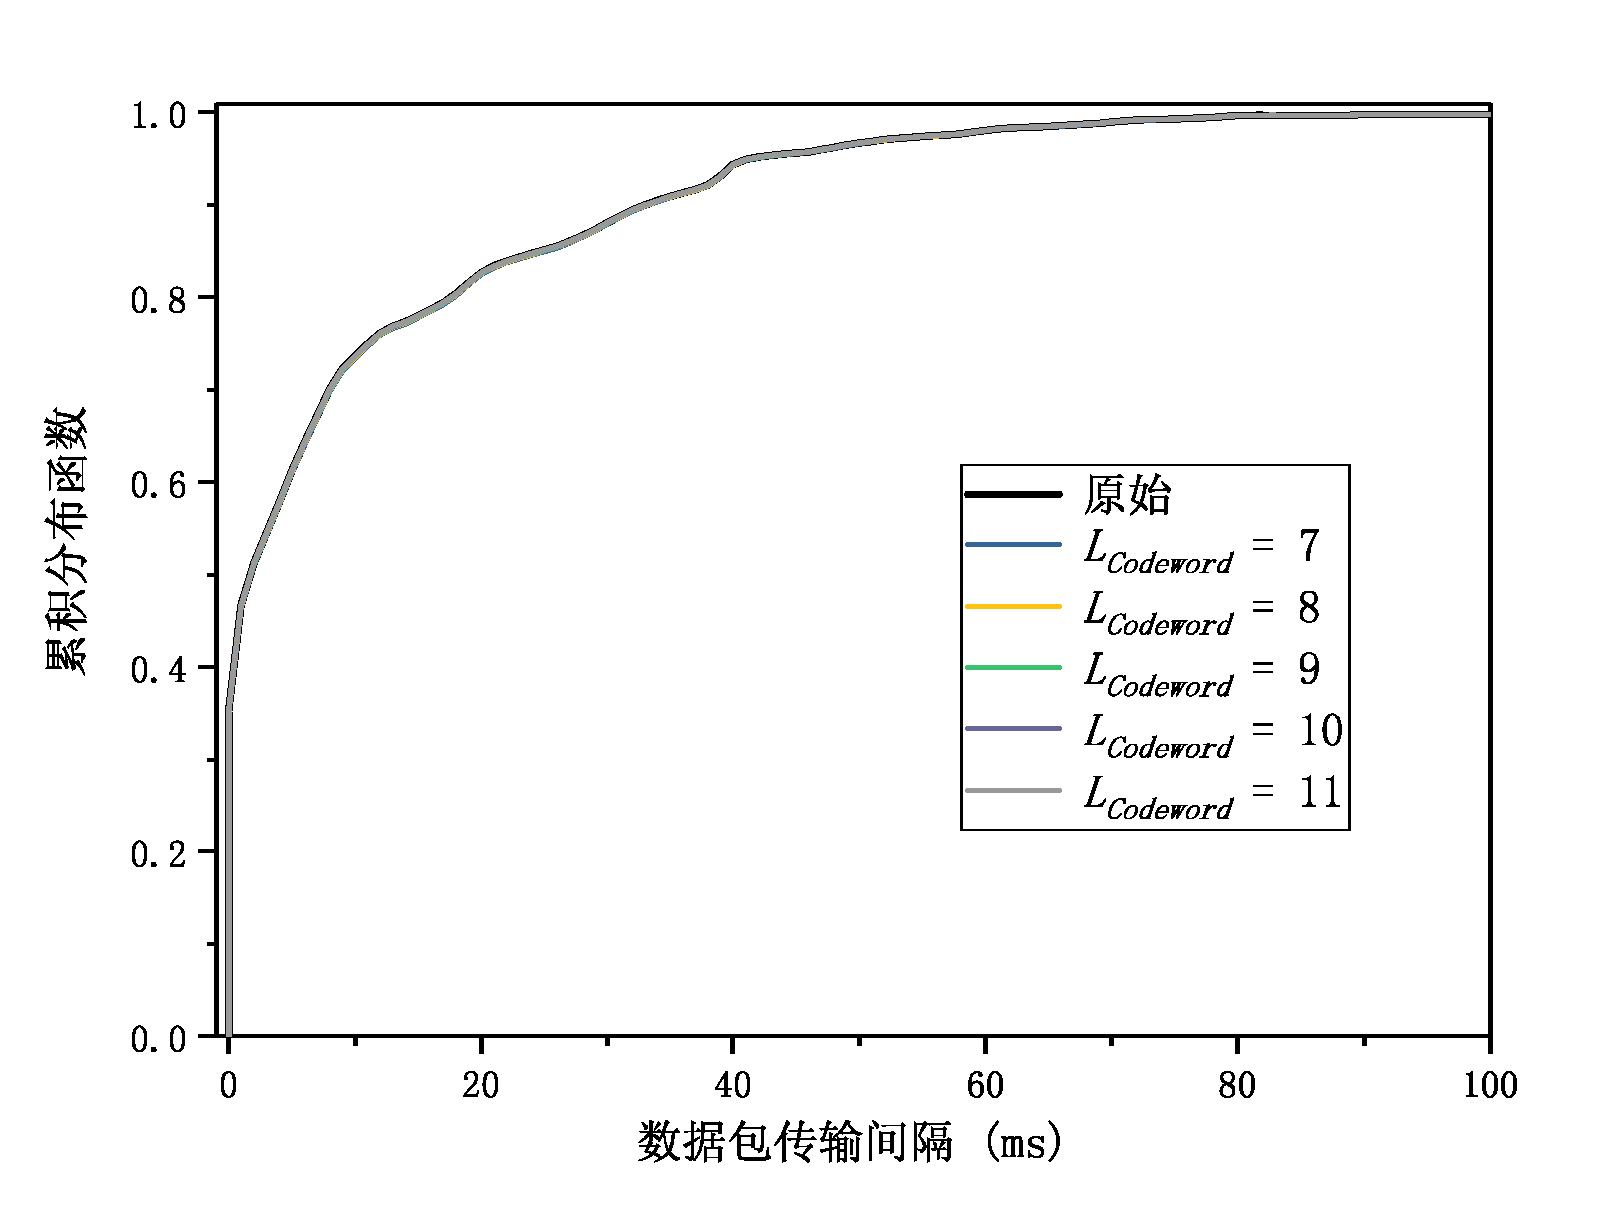
\includegraphics[width=0.48\textwidth]{chapters/chapter5/figures/ipd-cdf-excellent.pdf}
        }
        \subfigure[Good场景的CDF曲线]{
            \label{fig:5:result:ipd:cdf:good}
            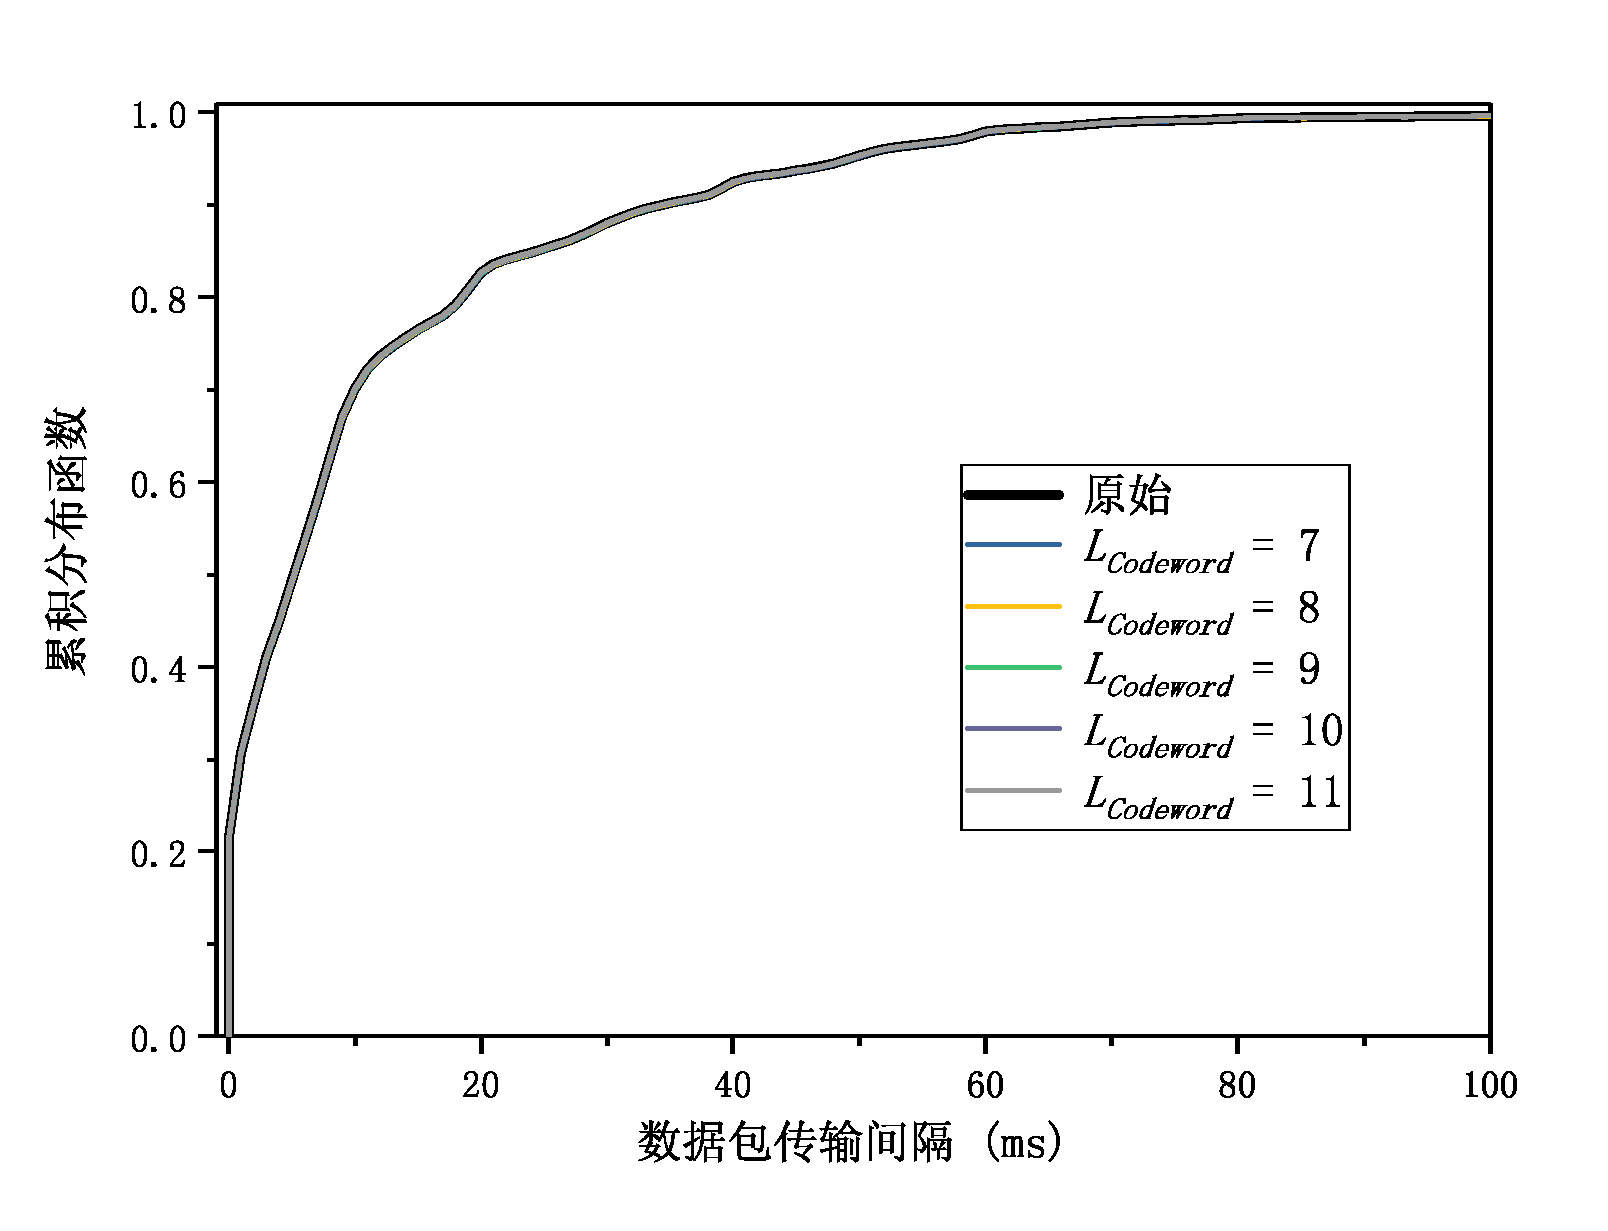
\includegraphics[width=0.48\textwidth]{chapters/chapter5/figures/ipd-cdf-good.pdf}
        }
        \caption{IPD分布的CDF曲线}
        \label{fig:5:result:ipd:cdf}
    \end{figure}
}

IPD分布的CDF曲线如图\ \nref{fig:5:result:ipd:cdf},时间隐通道对CDF分布无影响,该实验结果与本文\ \nref{chap:analyze:result:ipd:cdf}及本文\ \nref{chap:zigzag:results:undetectability:ipd}中得到的结果基本一致。当时间隐通道主动丢包率降低,对IPD分布的影响减小,CDF曲线已经无法检测到差异。

\insertTable{
	\begin{table}[htbp]
      \centering
      \caption{IPD检测检出率汇总表}
      \label{tab:5:result:ipd}
        \begin{threeparttable}
            \begin{tabular*}{0.85\textwidth}{@{\extracolsep{\fill}}ccc}
                \toprule
                $L_{Codeword}$ & 方法 & 检出率\\ 
                \midrule
                \multirow{5}{*}{7,8,9,10,11} 
                & K-S检验 & 0\ \% \\
                & Welch's t检验, Mann–Whitney rank检验\tnote{1} & 0\ \% \\
                & K-L散度 & 0\ \% \\
                & Wasserstein距离 & 0\ \% \\
                & 能量距离 & 0\ \% \\
                \bottomrule
            \end{tabular*}
            \begin{tablenotes}
                \footnotesize
                \item[1] Welch's t检验与Mann–Whitney rank检验通过一种即可
            \end{tablenotes}
        \end{threeparttable}
    \end{table}
}

IPD分布检测的量化评估结果如表\ \nref{tab:5:result:ipd},通过IPD分布无法检测出该时间隐通道。当前时间隐通道的检测方法,多基于IPD分布特征,因此已经具备良好抗检测能力。由于该时间隐通道的主动丢包率在{1\ \%}以内,具有足够的隐蔽性。

\subsubsection{连续丢包数检测}
\label{chap:hash:result:undetectability:burst}

\insertFigure{
    \begin{figure}[htbp]
        \centering
        \subfigure[Excellent场景的CDF曲线]{
            \label{fig:5:result:burst:cdf:excellent}
            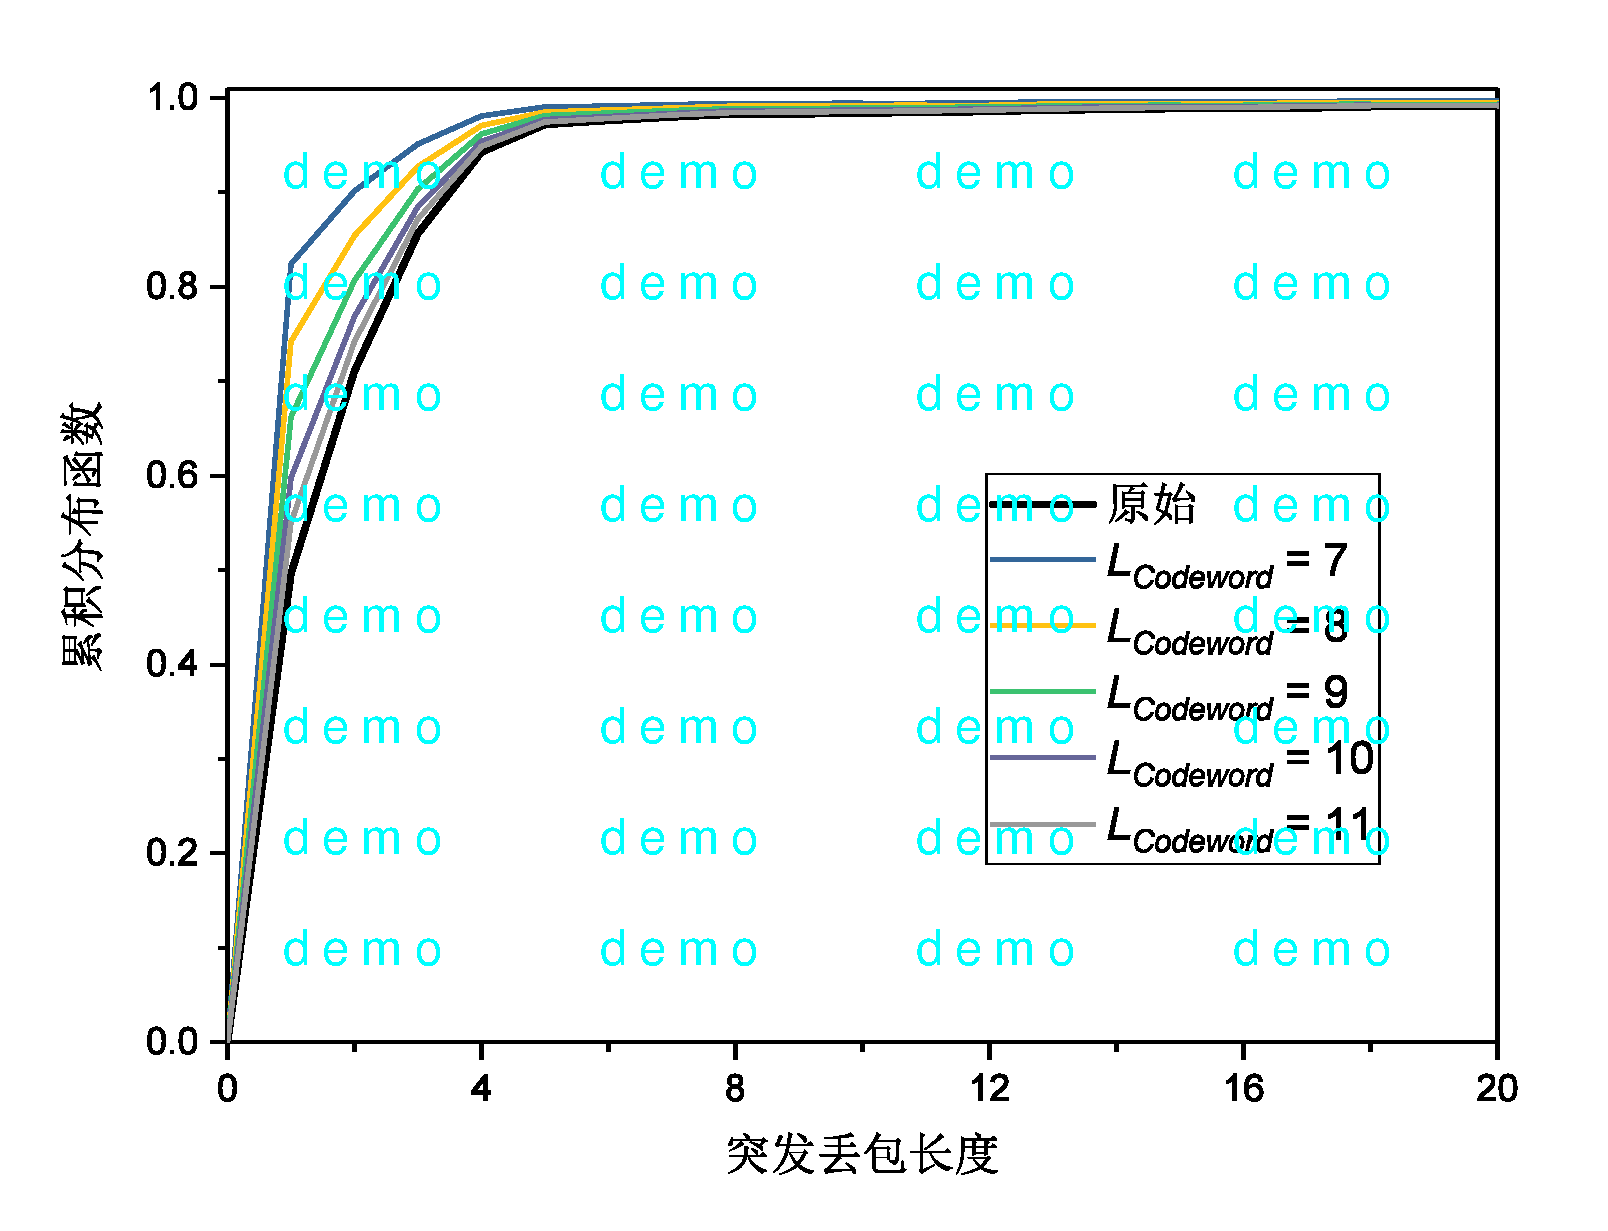
\includegraphics[width=0.48\textwidth]{chapters/chapter5/figures/burst-cdf-excellent.pdf}
        }
        \subfigure[Good场景的CDF曲线]{
            \label{fig:5:result:burst:cdf:good}
            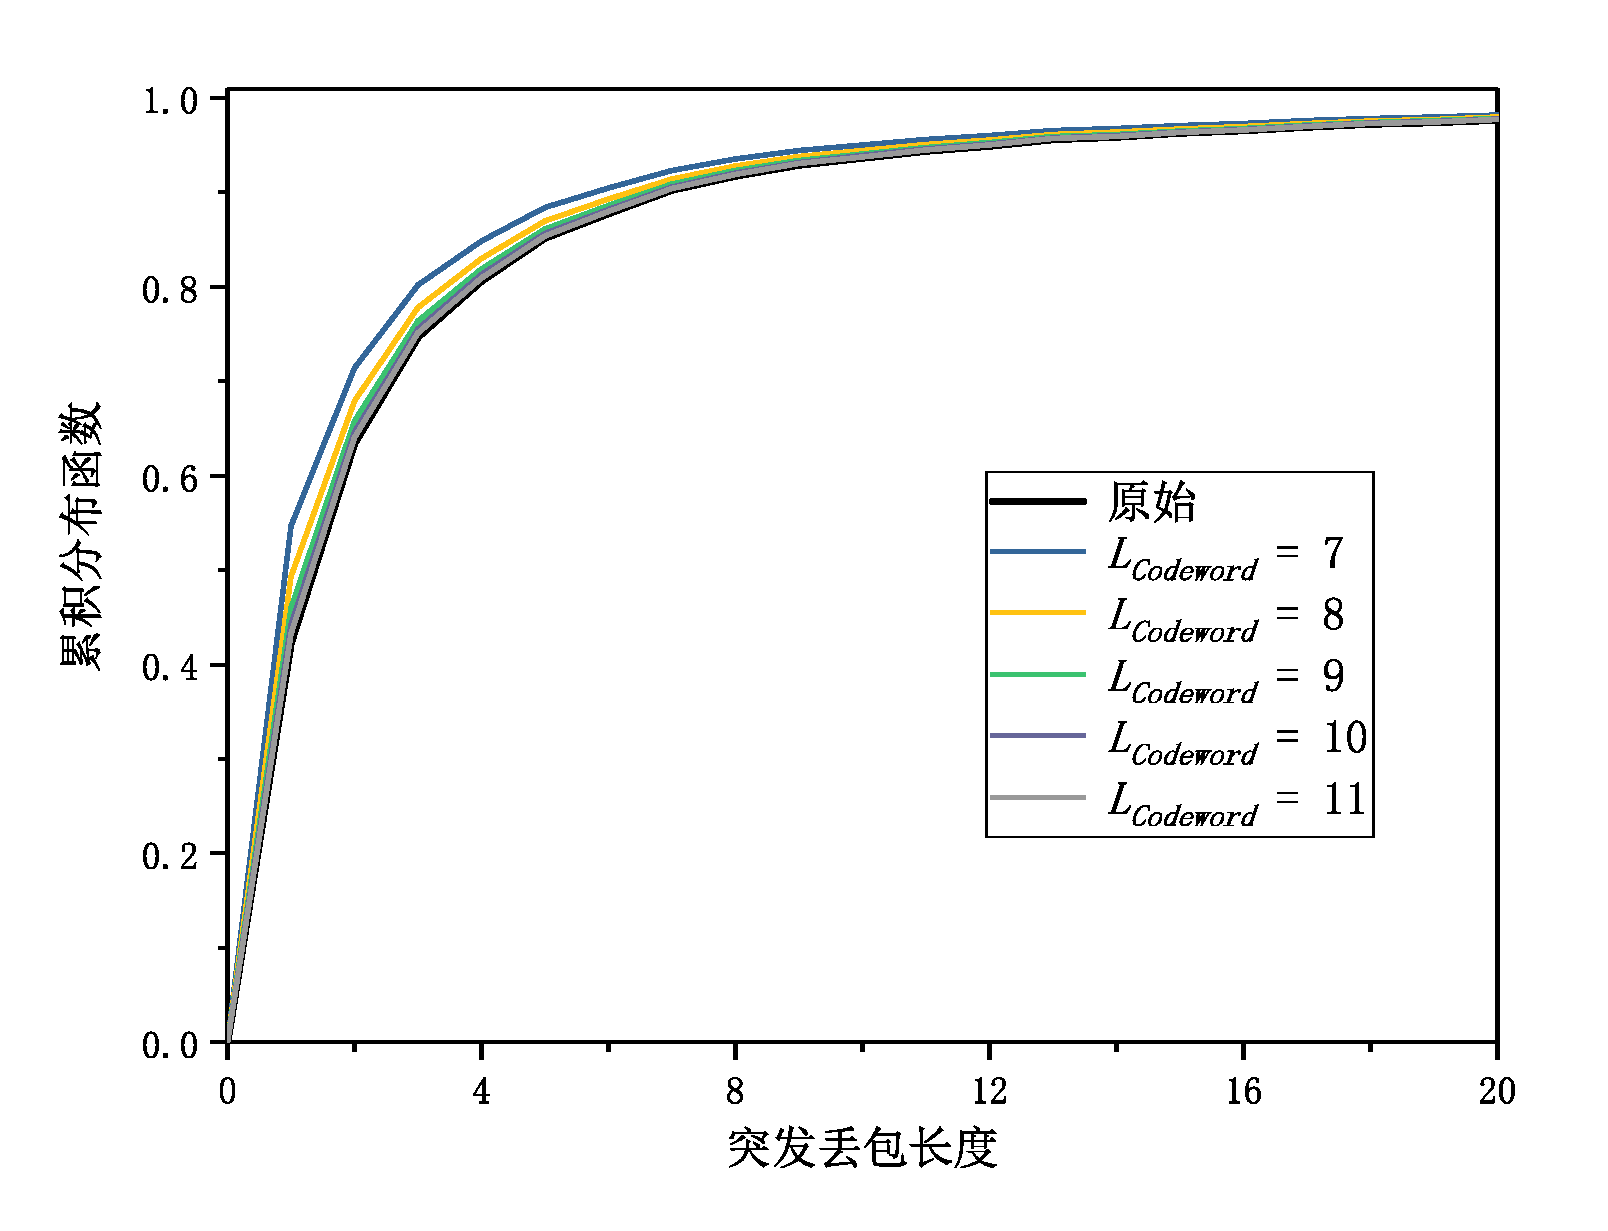
\includegraphics[width=0.48\textwidth]{chapters/chapter5/figures/burst-cdf-good.pdf}
        }
        \caption{连续丢包数的CDF曲线}
        \label{fig:5:result:burst:cdf}
    \end{figure}
}

连续丢包数反映了信道中的丢包类型,根据图\ \nref{fig:3:capture:burst:cdf},两种场景的主要区别为连续丢包所占比例。该方法中,主动丢包产生了长度为1的离散丢包。如图\ \nref{fig:5:result:burst:cdf},Excellent场景曲线出现偏离,而Good场景的曲线基本一致。由于Excellent场景网络噪声较弱,平均丢包率小于{1\ \%},时间隐通道对曲线存在影响;Good场景平均丢包率已经达到了{10\ \%}左右,而时间隐通道的主动丢包率小于{1\ \%},因此无影响。

\insertTable{
	\begin{table}[htbp]
      \centering
      \caption{连续丢包数检测检出率汇总表}
      \label{tab:5:result:burst}
          \begin{tabular*}{0.75\textwidth}{@{\extracolsep{\fill}}cccc}
            \toprule
            场景 & $L_{Codeword}$ & 方法 & 检出率 \\ 
            \midrule
            \multirow{4}{*}{Excellent} 
            & 7,8 & K-L散度 & 100\ \% \\
            & 9,10,11 & K-L散度 & 0\ \% \\
            & 7,8,9,10,11 & Wasserstein距离 & 0\ \% \\
            & 7,8,9,10,11 & 能量距离 & 0\ \% \\
            \\
            \multirow{3}{*}{Good}
            & 7,8,9,10,11 & K-L散度 & 0\ \% \\
            & 7,8,9,10,11 & Wasserstein距离 & 0\ \% \\
            & 7,8,9,10,11 & 能量距离 & 0\ \% \\
            \bottomrule
          \end{tabular*}
    \end{table}
}

连续丢包数检测的量化评估结果如表\ \nref{tab:5:result:burst},Good场景下具有较好的隐蔽性,当$L_{Codeword}\ge 7$时通过了所有的检测。Excellent场景下,参数$L_{Codeword}\ge 9$时,才能通过所有的检测项。因此,要保证该时间隐通道具备全场景抗检测能力,参数$L_{Codeword}$应当满足$L_{Codeword}\ge 9$。

\subsubsection{区间丢包数检测}
\label{chap:hash:result:undetectability:plr}

\insertFigure{
    \begin{figure}[htbp]
        \centering
        \subfigure[区间长度为100时Excellent场景的CDF曲线]{
            \label{fig:5:result:win100:cdf:excellent}
            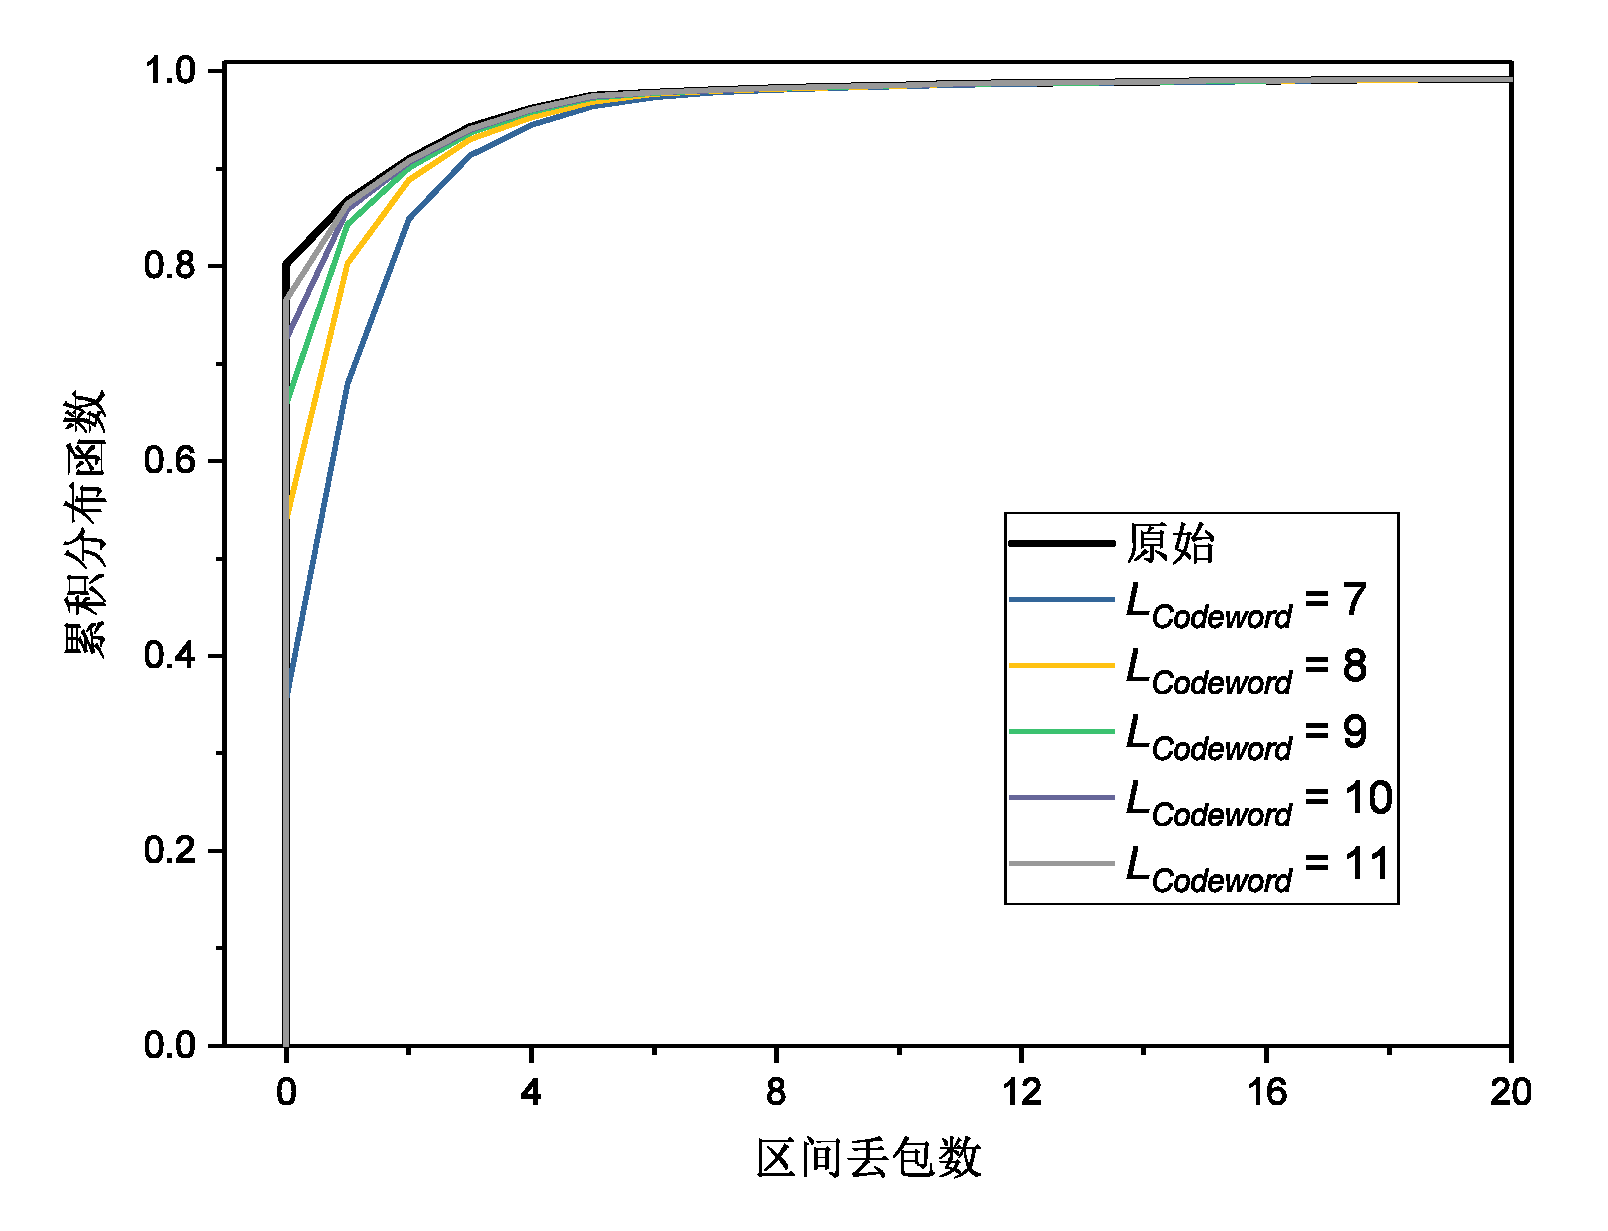
\includegraphics[width=0.48\textwidth]{chapters/chapter5/figures/win100-cdf-excellent.pdf}
        }
        \subfigure[区间长度为100时Good场景的CDF曲线]{
            \label{fig:5:result:win100:cdf:good}
            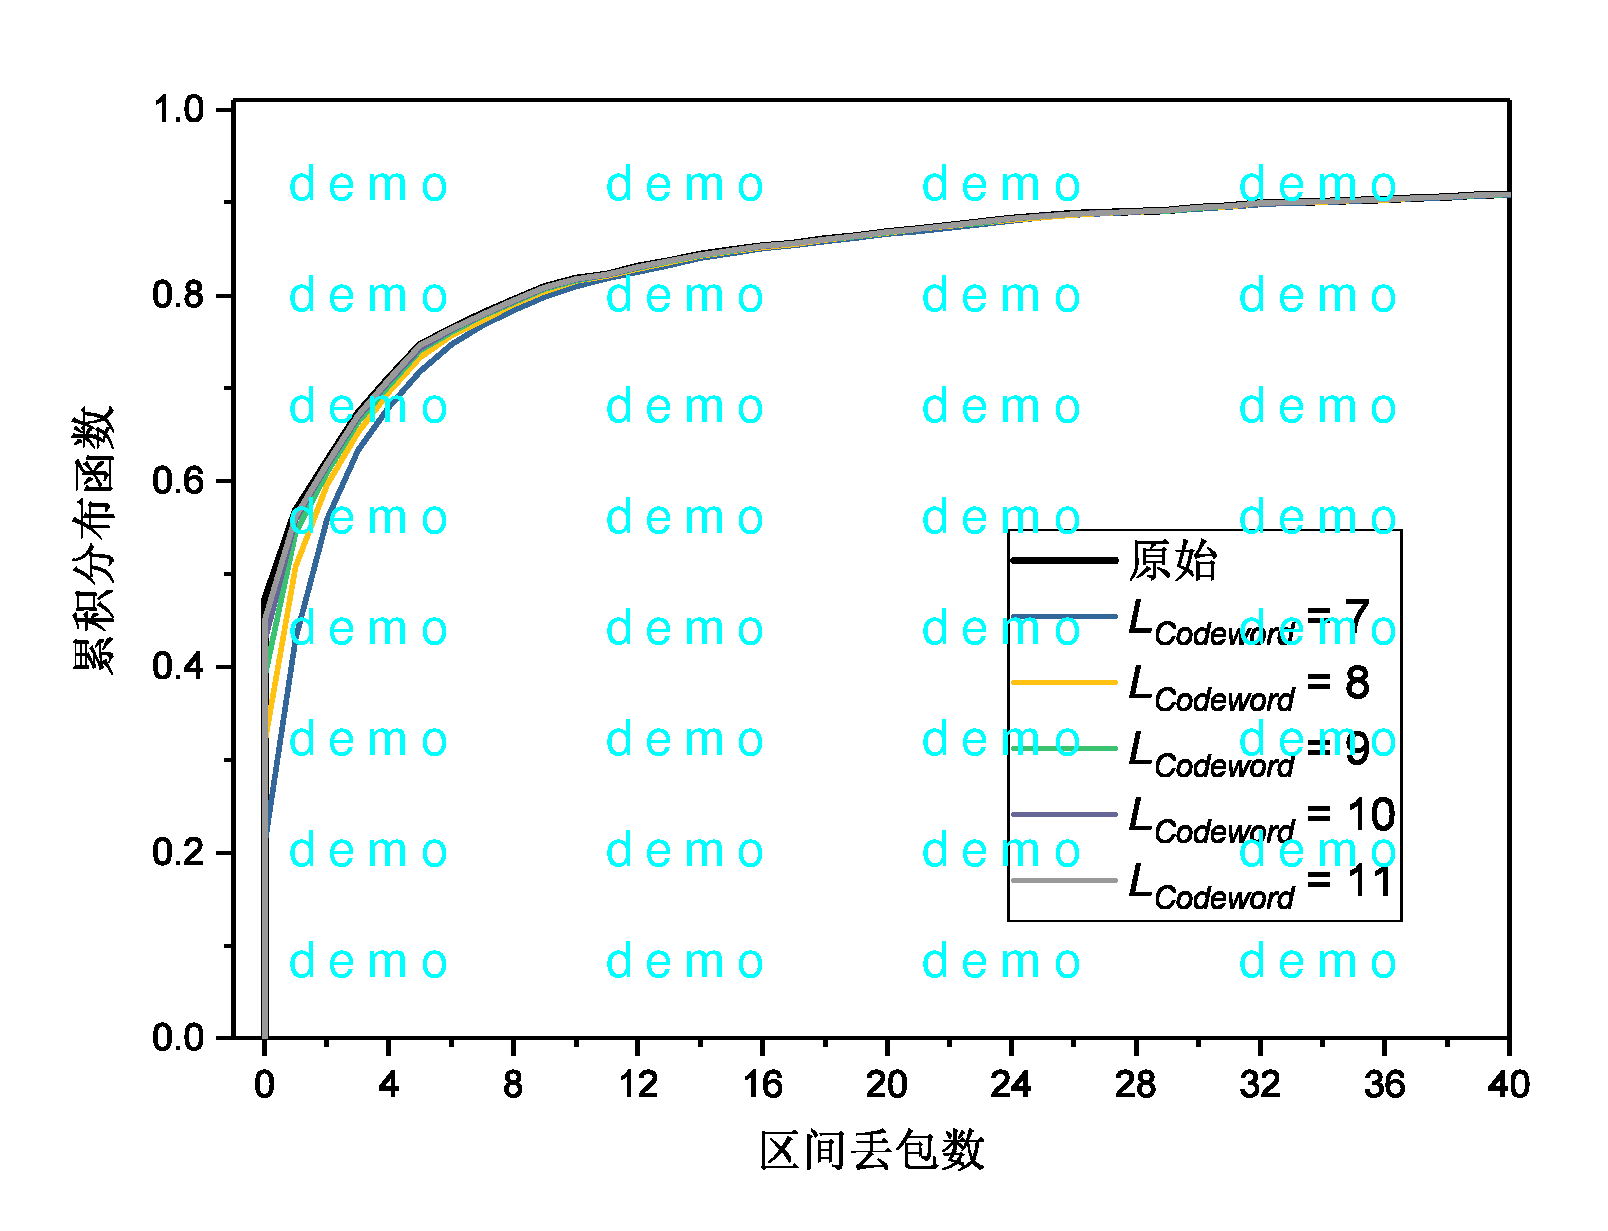
\includegraphics[width=0.48\textwidth]{chapters/chapter5/figures/win100-cdf-good.pdf}
        }
        \subfigure[区间长度为200时Excellent场景的CDF曲线]{
            \label{fig:5:result:win200:cdf:excellent}
            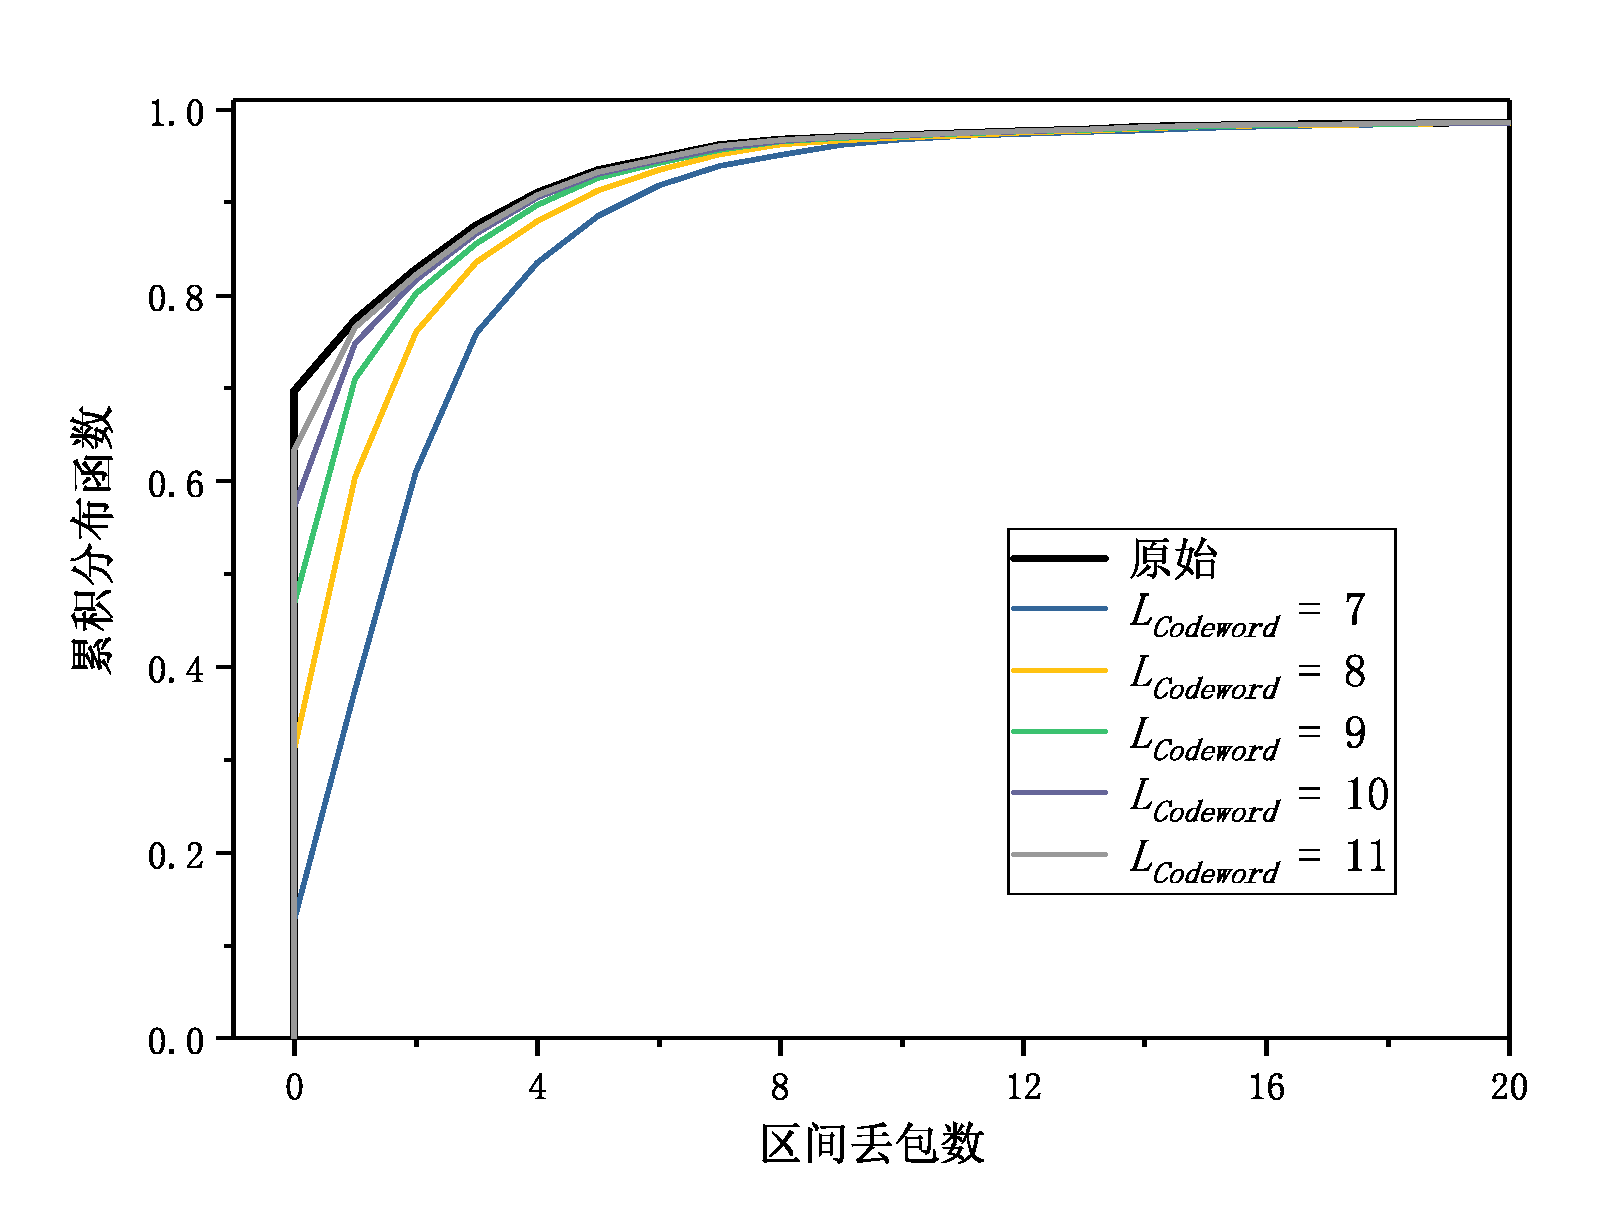
\includegraphics[width=0.48\textwidth]{chapters/chapter5/figures/win200-cdf-excellent.pdf}
        }
        \subfigure[区间长度为200时Good场景的CDF曲线]{
            \label{fig:5:result:win200:cdf:good}
            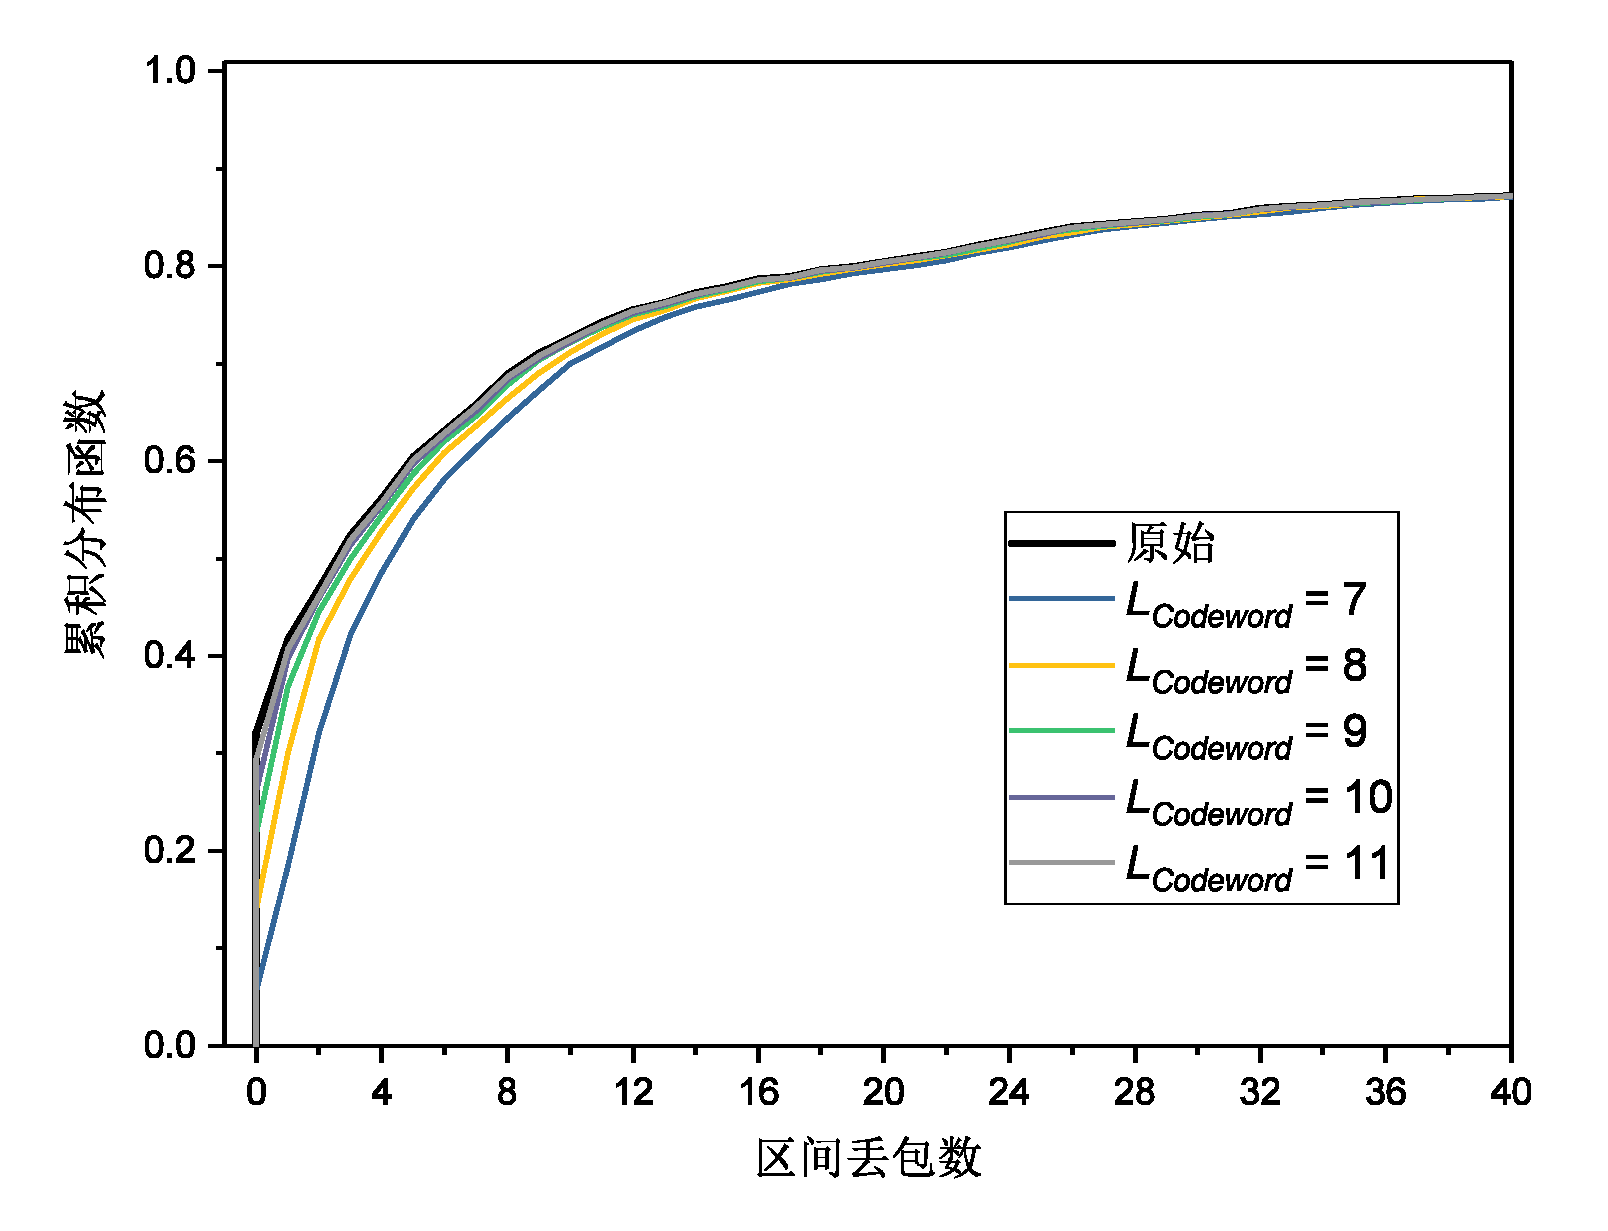
\includegraphics[width=0.48\textwidth]{chapters/chapter5/figures/win200-cdf-good.pdf}
        }
        \caption{区间丢包数的CDF曲线}
        \label{fig:5:result:win:cdf}
    \end{figure}
}

基于主动丢包的时间隐通道,存在固定区间内的丢包行为,对区间丢包数产生影响。区间丢包数的CDF曲线如图\ \nref{fig:5:result:win:cdf},区间长度设定为100及200。Excellent场景如图\ \nref{fig:5:result:win100:cdf:excellent}及图\ \nref{fig:5:result:win200:cdf:excellent},时间隐通道的CDF曲线已经出现偏离,并且随着$L_{Codeword}$减小,相对偏离增大。Good场景如图\ \nref{fig:5:result:win100:cdf:good}及图\ \nref{fig:5:result:win200:cdf:good},时间隐通道的相对偏离较小,具有更好的隐蔽性。

\insertTable{
	\begin{table}[htbp]
      \centering
      \caption{区间丢包数检测检出率汇总表}
      \label{tab:5:result:win}
          \begin{tabular*}{0.75\textwidth}{@{\extracolsep{\fill}}cccc}
            \toprule
            场景 & $L_{Codeword}$ & 方法 & 检出率 \\ 
            \midrule
            \multirow{4}{*}{Excellent} 
            & 7 & Wasserstein距离 & 100\ \% \\
            & 8,9,10,11 & Wasserstein距离 & 0\ \% \\
            & 7 & 能量距离 & 100\ \% \\
            & 8,9,10,11 & 能量距离 & 0\ \% \\
            \\
            \multirow{6}{*}{Good}
            & 7 & Wasserstein距离 & 100\ \% \\
            & 8 & Wasserstein距离 & 30\ \% \\
            & 9,10,11 & Wasserstein距离 & 0\ \% \\
            & 7 & 能量距离 & 100\ \% \\
            & 8 & 能量距离 & 30\ \% \\
            & 9,10,11 & 能量距离 & 0\ \% \\
            \bottomrule
          \end{tabular*}
    \end{table}
}

区间丢包数检测的量化评估结果如表\ \nref{tab:5:result:win},检出结果与本文\ \nref{tab:4:results:win}类似。Excellent场景下,当$L_{Codeword}\ge 8$时,该时间隐通道即可通过检测;Good场景下,当$L_{Codeword}\ge 9$时,该时间隐通道通过所有检测;当$L_{Codeword}=8$时,该时间隐通道有较高几率通过检测。

\subsubsection{抗检测能力测试汇总}
\label{chap:hash:result:undetectability:sum}

\insertTable{
	\begin{table}[htbp]
      \centering
      \caption{基于多重校验纠错的时间隐通道检出率汇总表}
      \label{tab:5:result:sum}
          \begin{tabular*}{0.8\textwidth}{@{\extracolsep{\fill}}cccccc}
            \toprule
            \multirow{2}{*}{场景} 
            & \multicolumn{5}{c}{$L_{Codeword}$} \\
            \cmidrule(l){2-6}
            & 7 & 8 & 9 & 10 & 11 \\
            \midrule
            Excellent & 100\ \% & 100\ \% & 0\ \% & 0\ \% & 0\ \% \\
            Good & 100\ \% & 30\ \% & 0\ \% & 0\ \% & 0\ \% \\
            \bottomrule
          \end{tabular*}
    \end{table}
}

根据表\ \nref{tab:3:detect-sum}中的所有检测项,该时间隐通道的检出率汇总如表\ \nref{tab:5:result:sum}。Good场景中,该方法具有较好的隐蔽性,当$L_{Codeword}\ =\ 8$时仍有较高几率通过检测。要通过所有场景下的所有测试,参数$L_{Codeword}$应当满足$L_{Codeword}\ge 9$。

\subsection{鲁棒性测试}
\label{chap:hash:result:robustness}

鲁棒性测试的评估指标是误码率,计算方法如公式(\nref{equ:2:ber})。该时间隐通道中,影响误码率的参数包括$L_{Codeword}$、$L_{HASH}$、$L_{CRC}$、$R$及$M_{cols}$,因此鲁棒性评估主要围绕这五个参数进行。在测试数据集方面,除了Excellent场景及Good场景,还设置了四种不同比例的随机丢包场景。

\insertFigure{
	\begin{figure}[htb]
        \centering
        \subfigure[Excellent场景的平均误码率]{
            \label{fig:5:result:ber:mcols:excellent}
            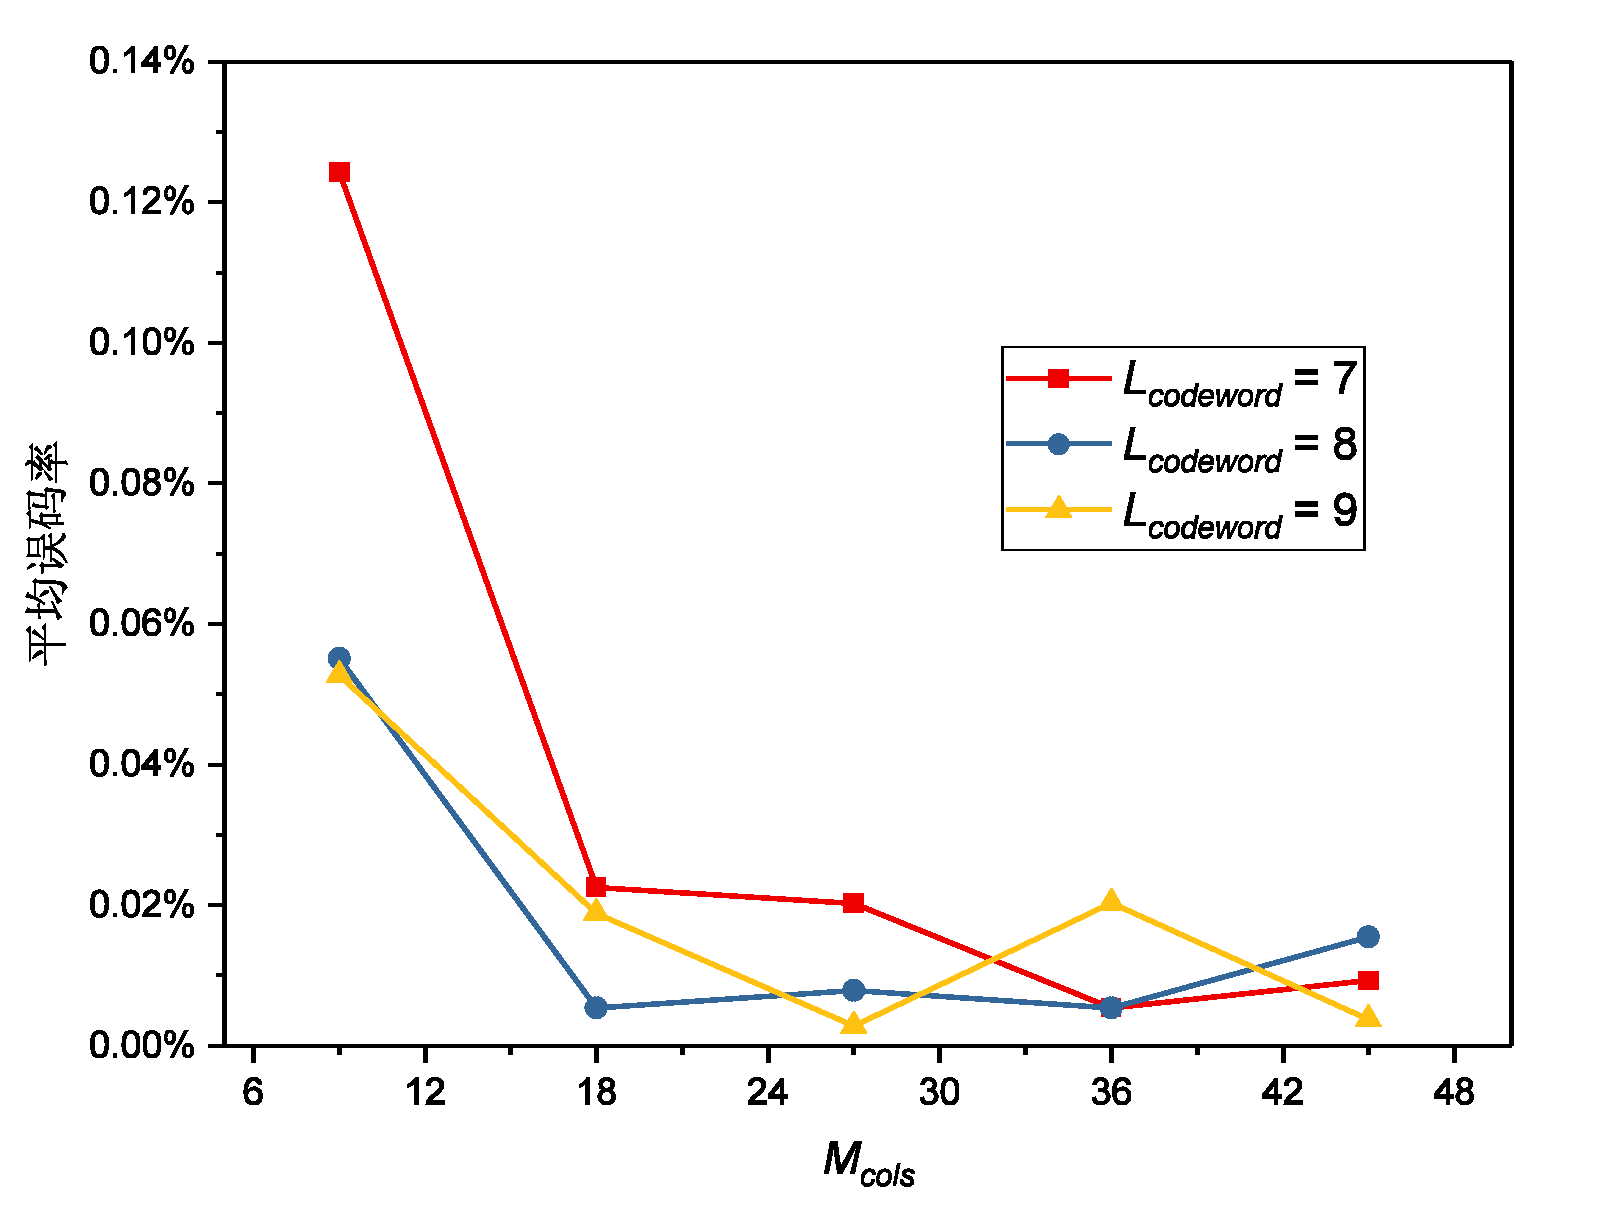
\includegraphics[width=0.48\textwidth]{chapters/chapter5/figures/ber-mcols-excellent.pdf}
        }
        \subfigure[Good场景的平均误码率]{
            \label{fig:5:result:ber:mcols:good}
            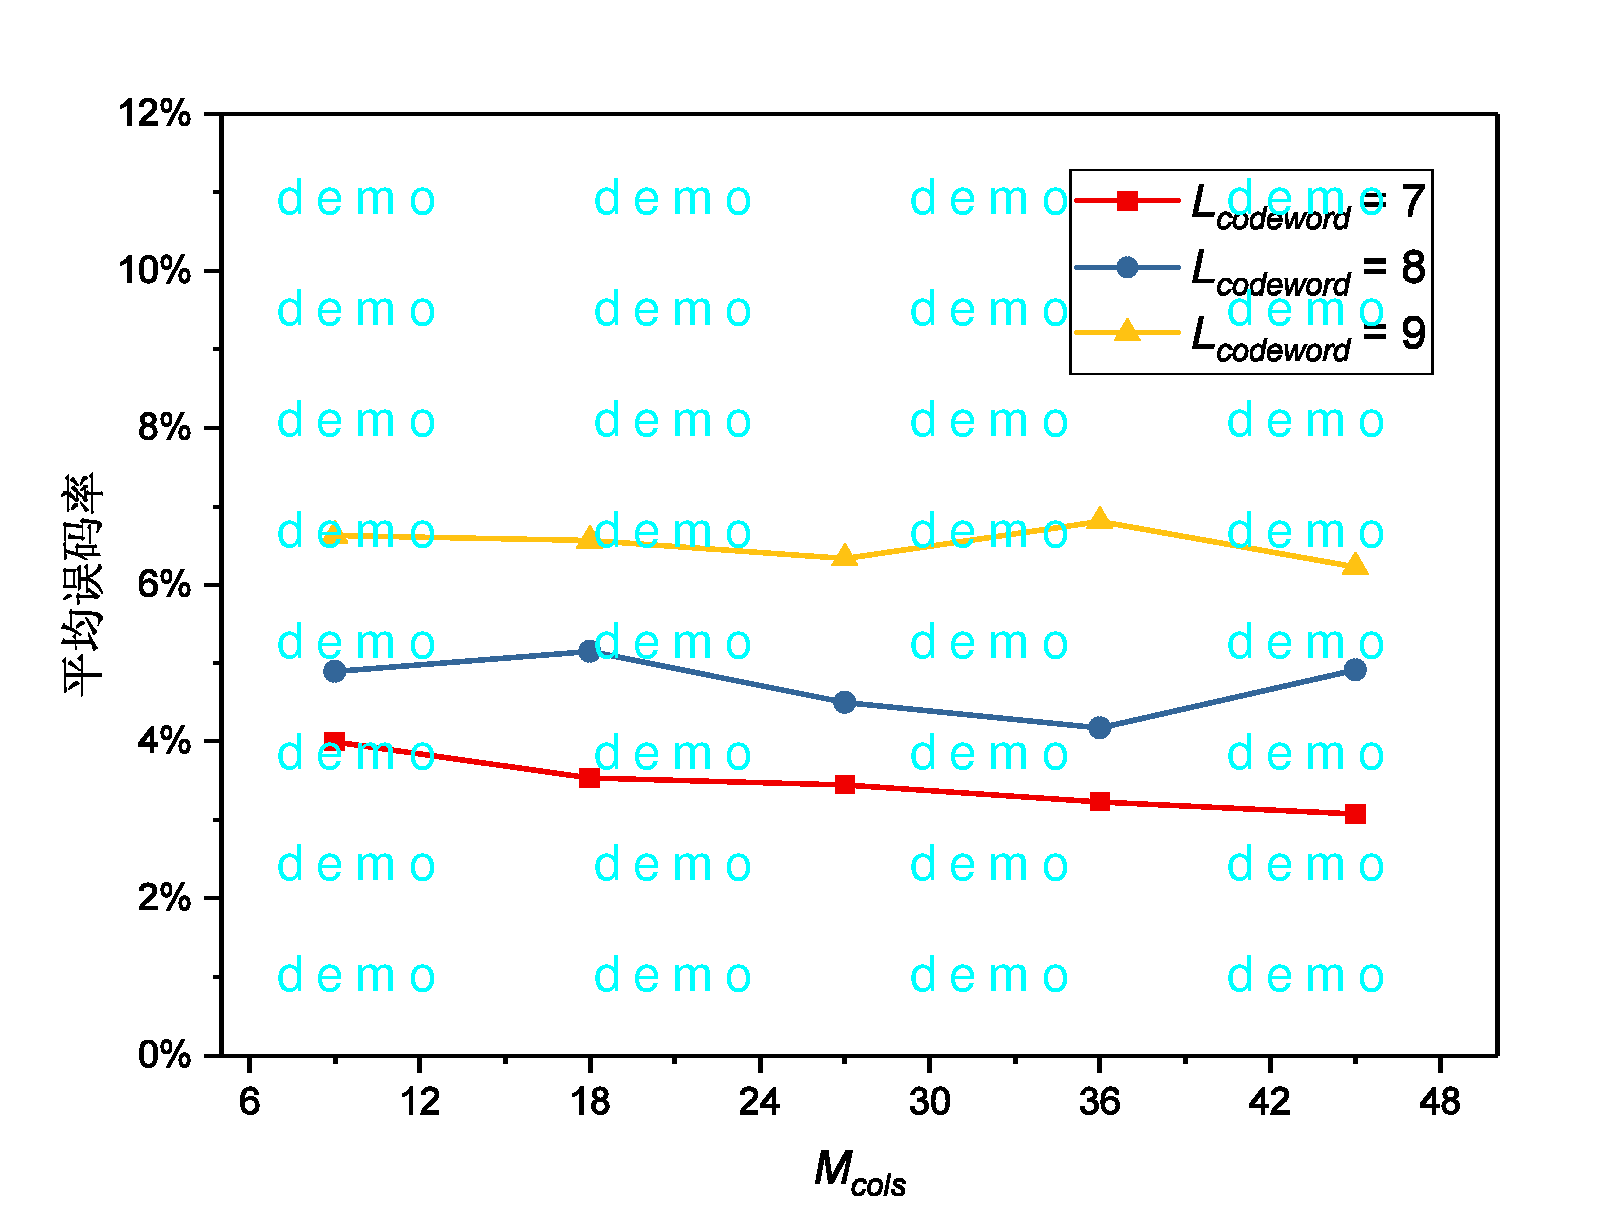
\includegraphics[width=0.48\textwidth]{chapters/chapter5/figures/ber-mcols-good.pdf}
        }
        \caption{平均误码率与$M_{cols}$的折线图}
        \label{fig:5:result:ber:mcols}
    \end{figure}

    \begin{figure}[htb]
        \centering
        \subfigure[Excellent场景的平均误码率]{
            \label{fig:5:result:ber:lcodeword:excellent}
            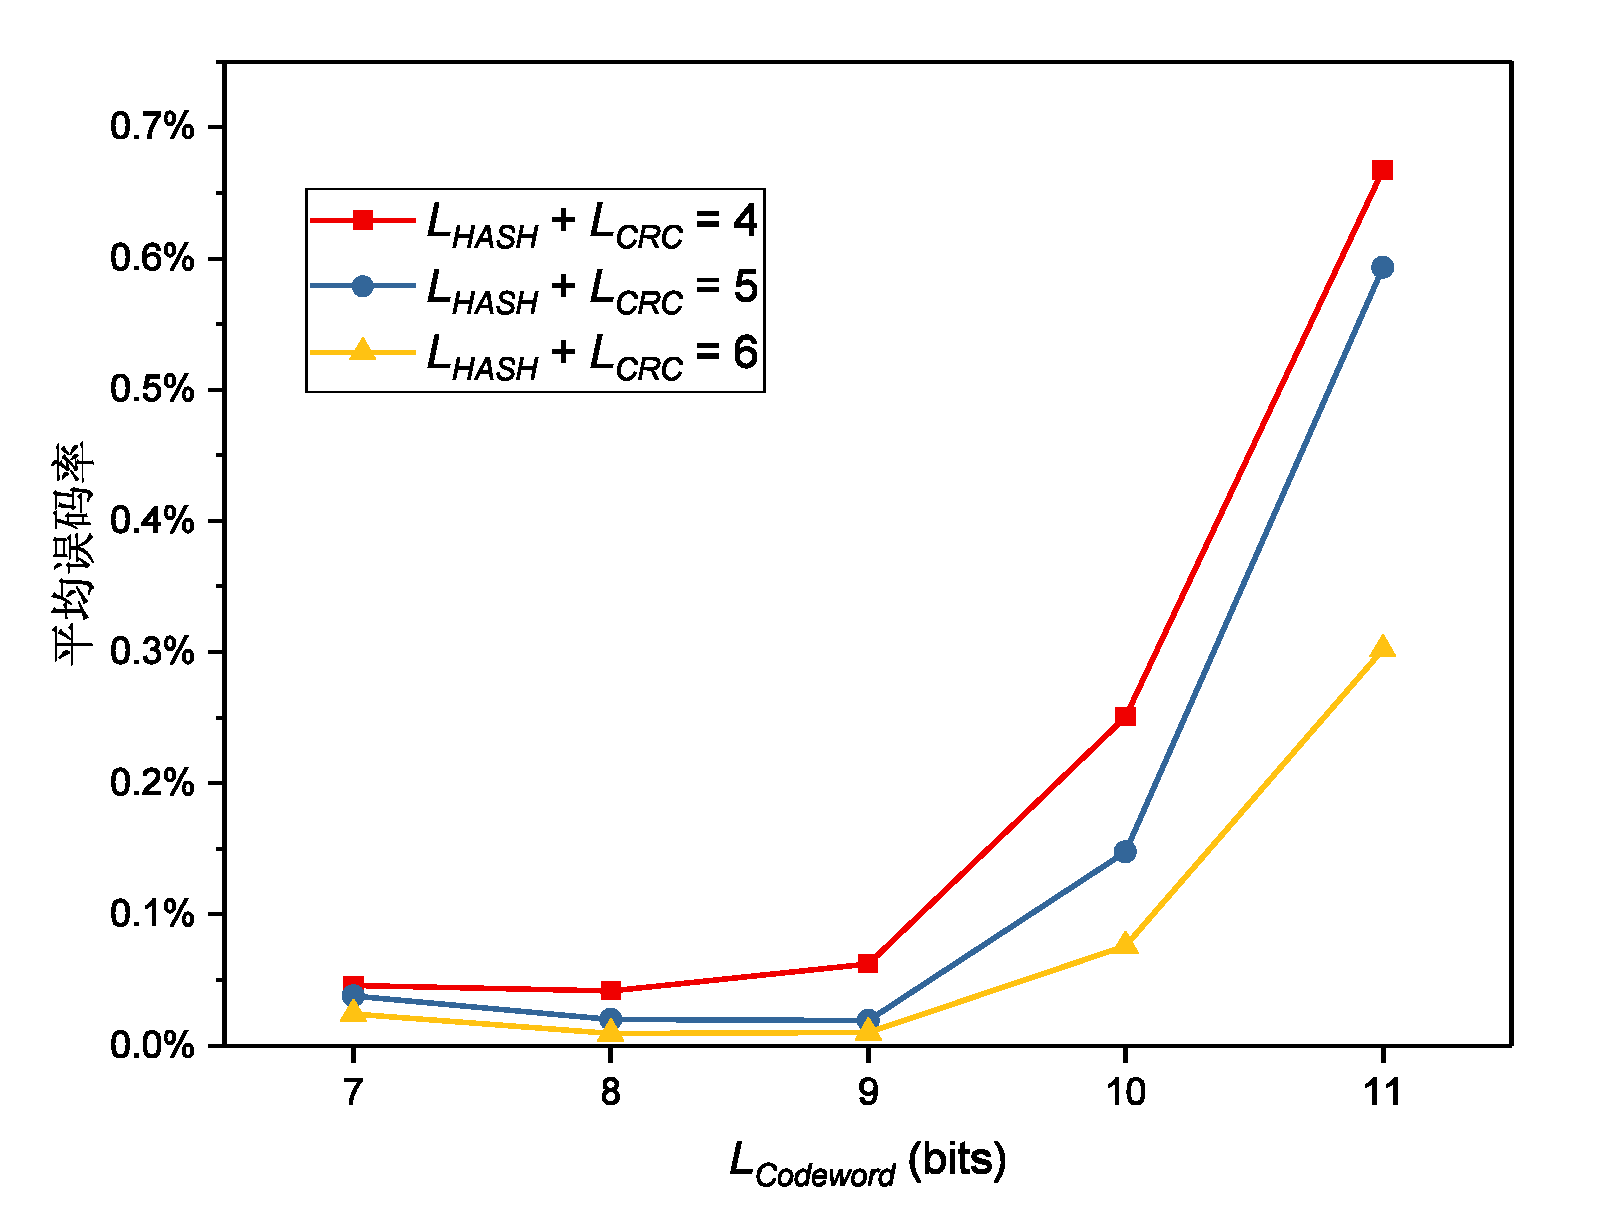
\includegraphics[width=0.48\textwidth]{chapters/chapter5/figures/ber-lcodeword-excellent.pdf}
        }
        \subfigure[Good场景的平均误码率]{
            \label{fig:5:result:ber:lcodeword:good}
            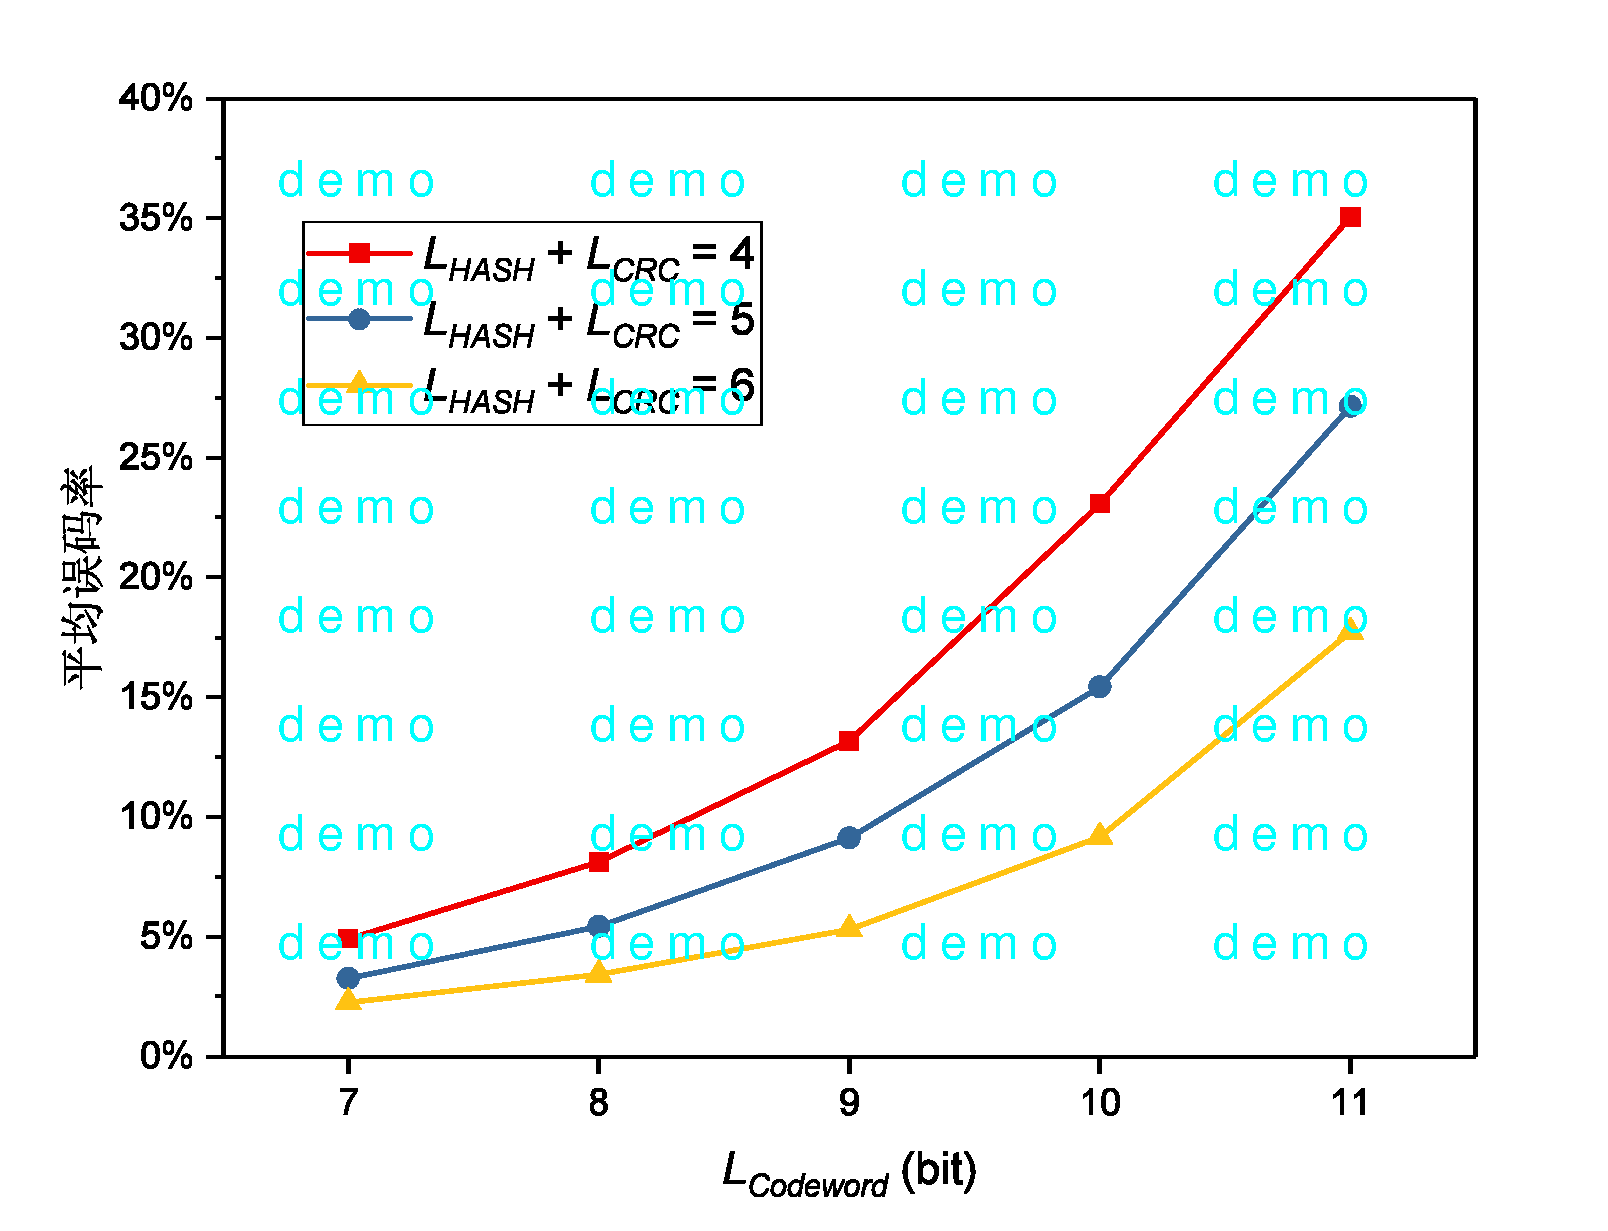
\includegraphics[width=0.48\textwidth]{chapters/chapter5/figures/ber-lcodeword-good.pdf}
        }
        \caption{平均误码率与$L_{Codeword}$的折线图}
        \label{fig:5:result:ber:lcodeword}
    \end{figure}

    \begin{figure}[htb]
        \centering
        \subfigure[Excellent场景的平均误码率]{
            \label{fig:5:result:ber:lhash:excellent}
            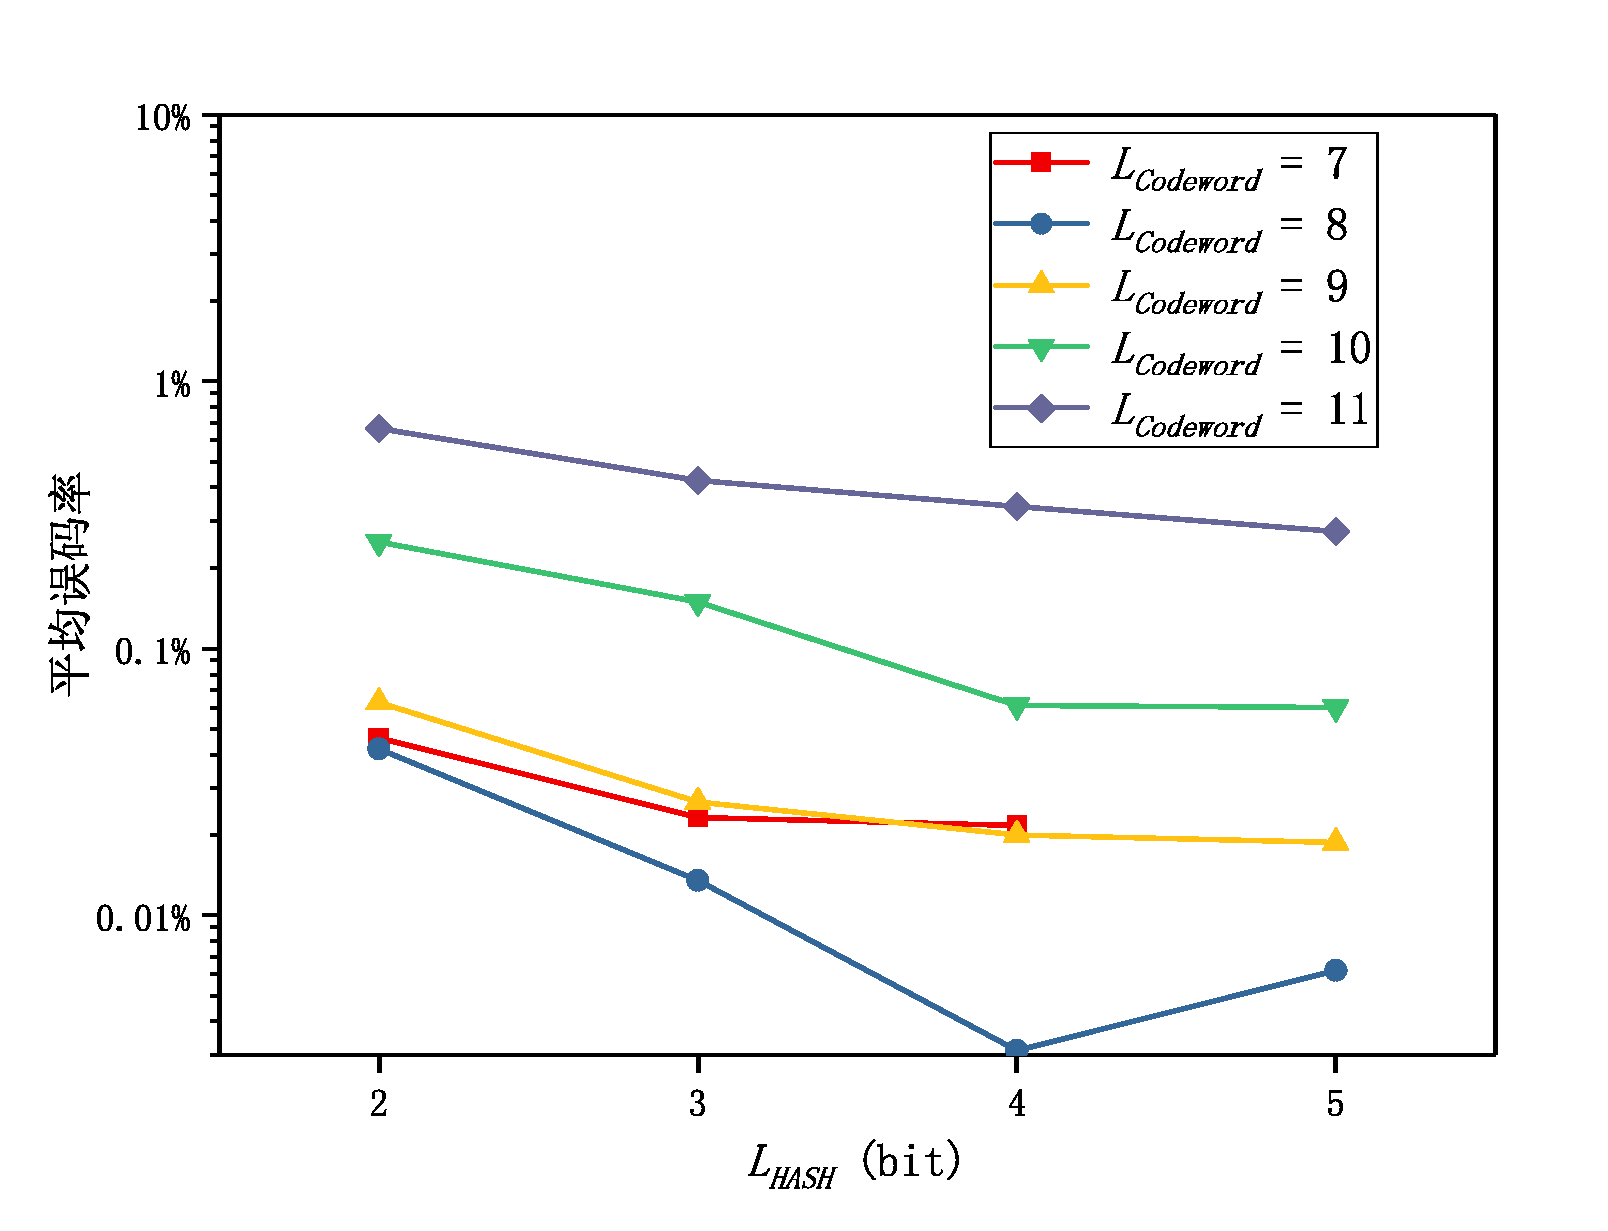
\includegraphics[width=0.48\textwidth]{chapters/chapter5/figures/ber-lhash-excellent.pdf}
        }
        \subfigure[Good场景的平均误码率]{
            \label{fig:5:result:ber:lhash:good}
            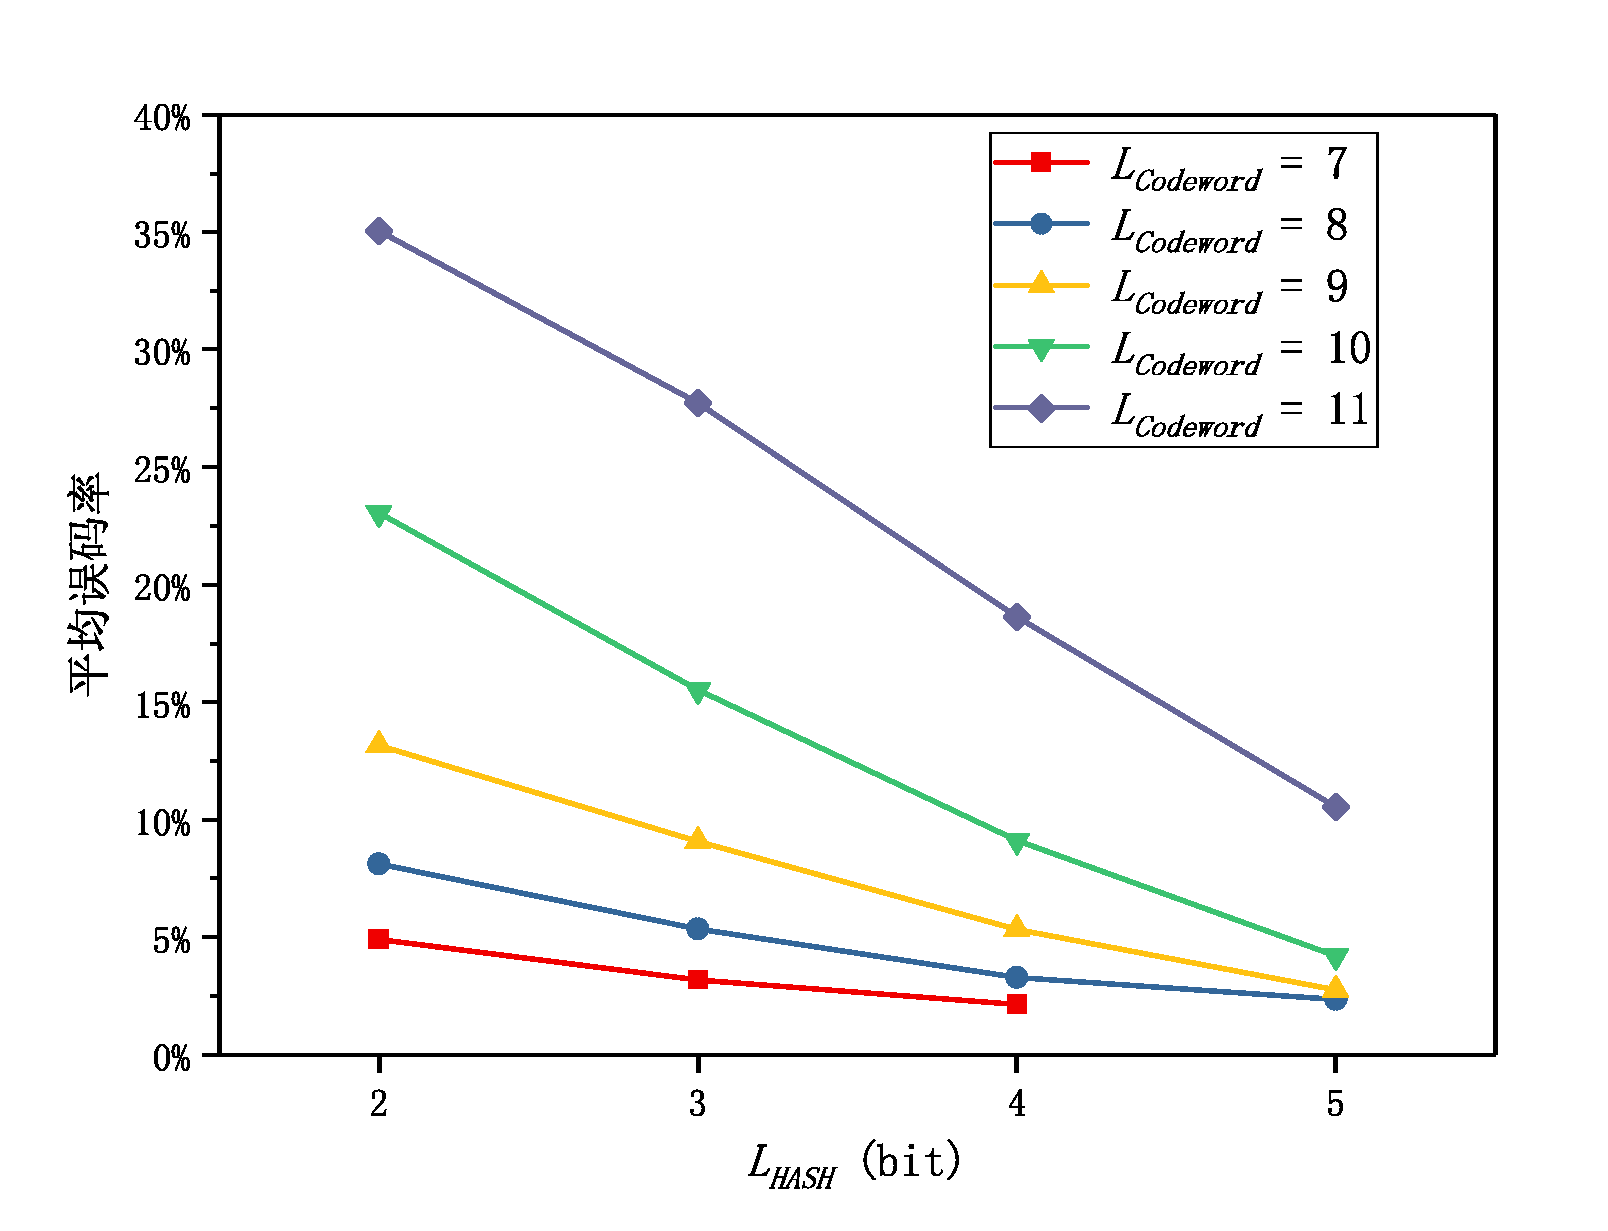
\includegraphics[width=0.48\textwidth]{chapters/chapter5/figures/ber-lhash-good.pdf}
        }
        \caption{平均误码率与$L_{HASH}$的折线图}
        \label{fig:5:result:ber:lhash}
    \end{figure}

    \begin{figure}[htb]
        \centering
        \subfigure[Excellent场景的平均误码率]{
            \label{fig:5:result:ber:lcrc:excellent}
            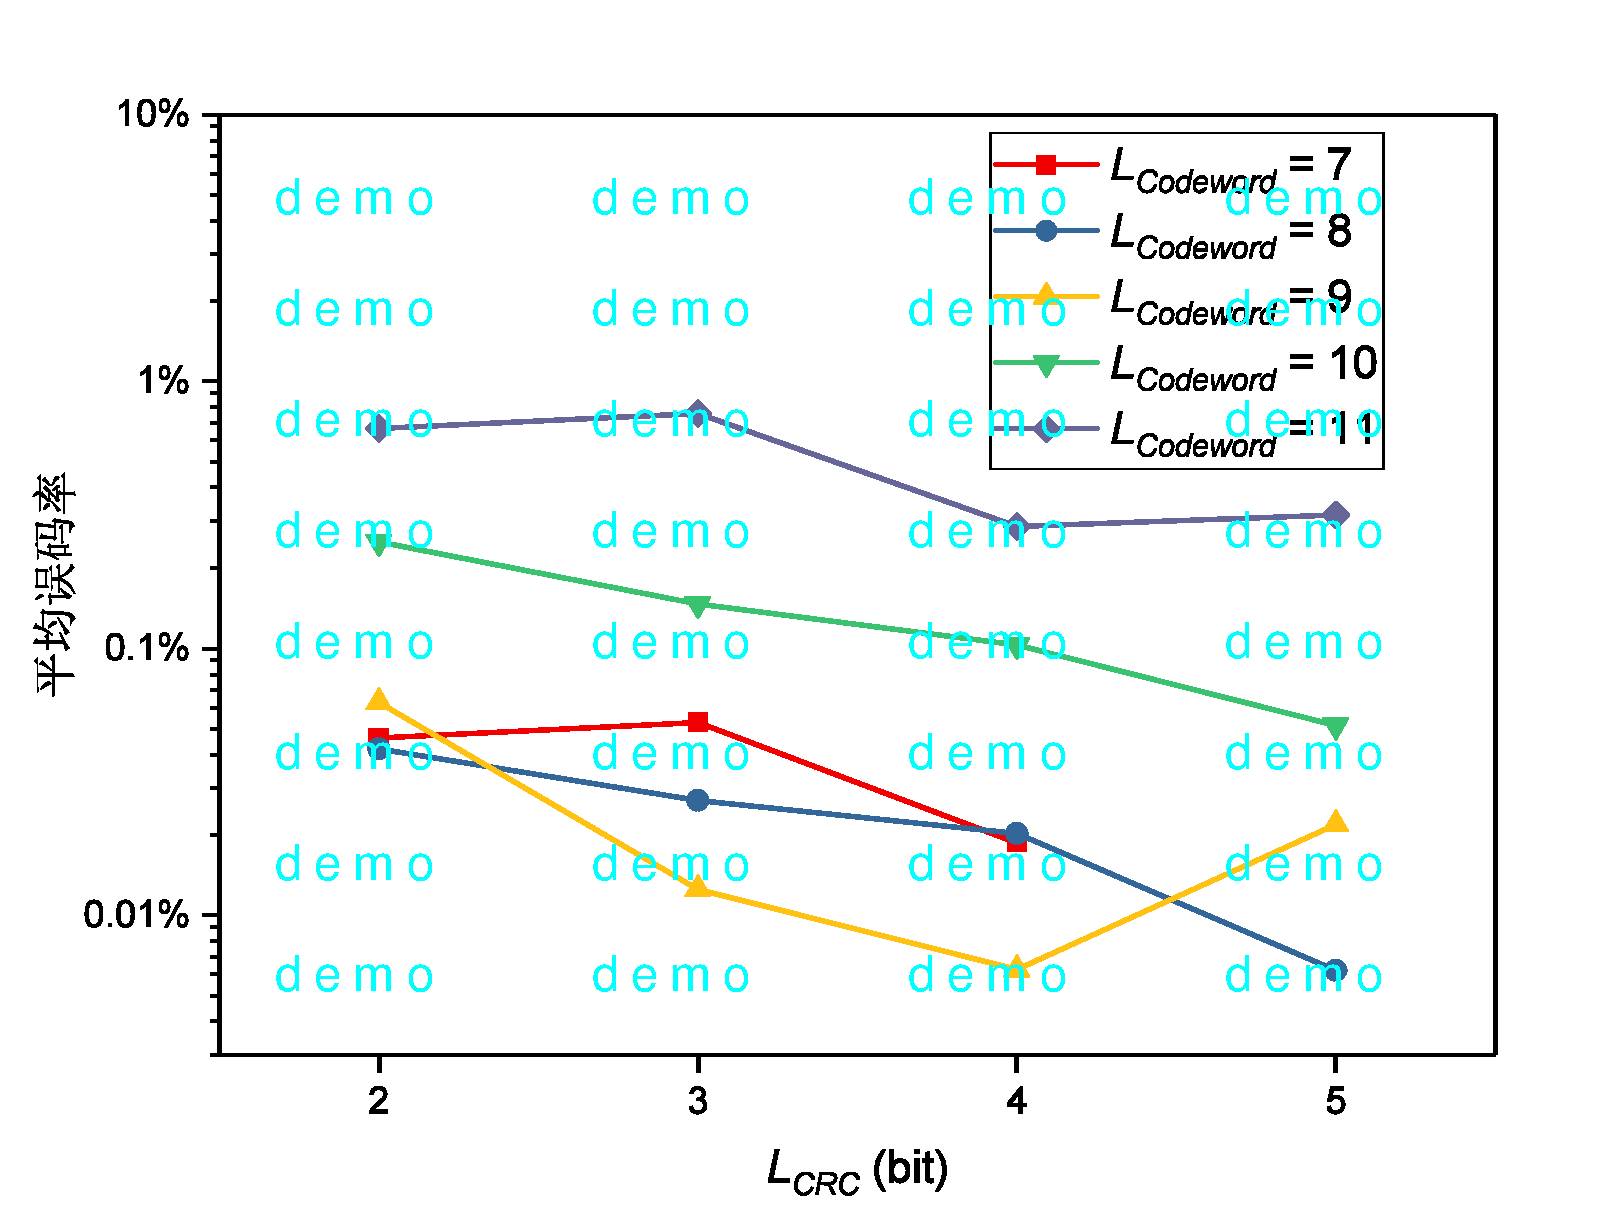
\includegraphics[width=0.48\textwidth]{chapters/chapter5/figures/ber-lcrc-excellent.pdf}
        }
        \subfigure[Good场景的平均误码率]{
            \label{fig:5:result:ber:lcrc:good}
            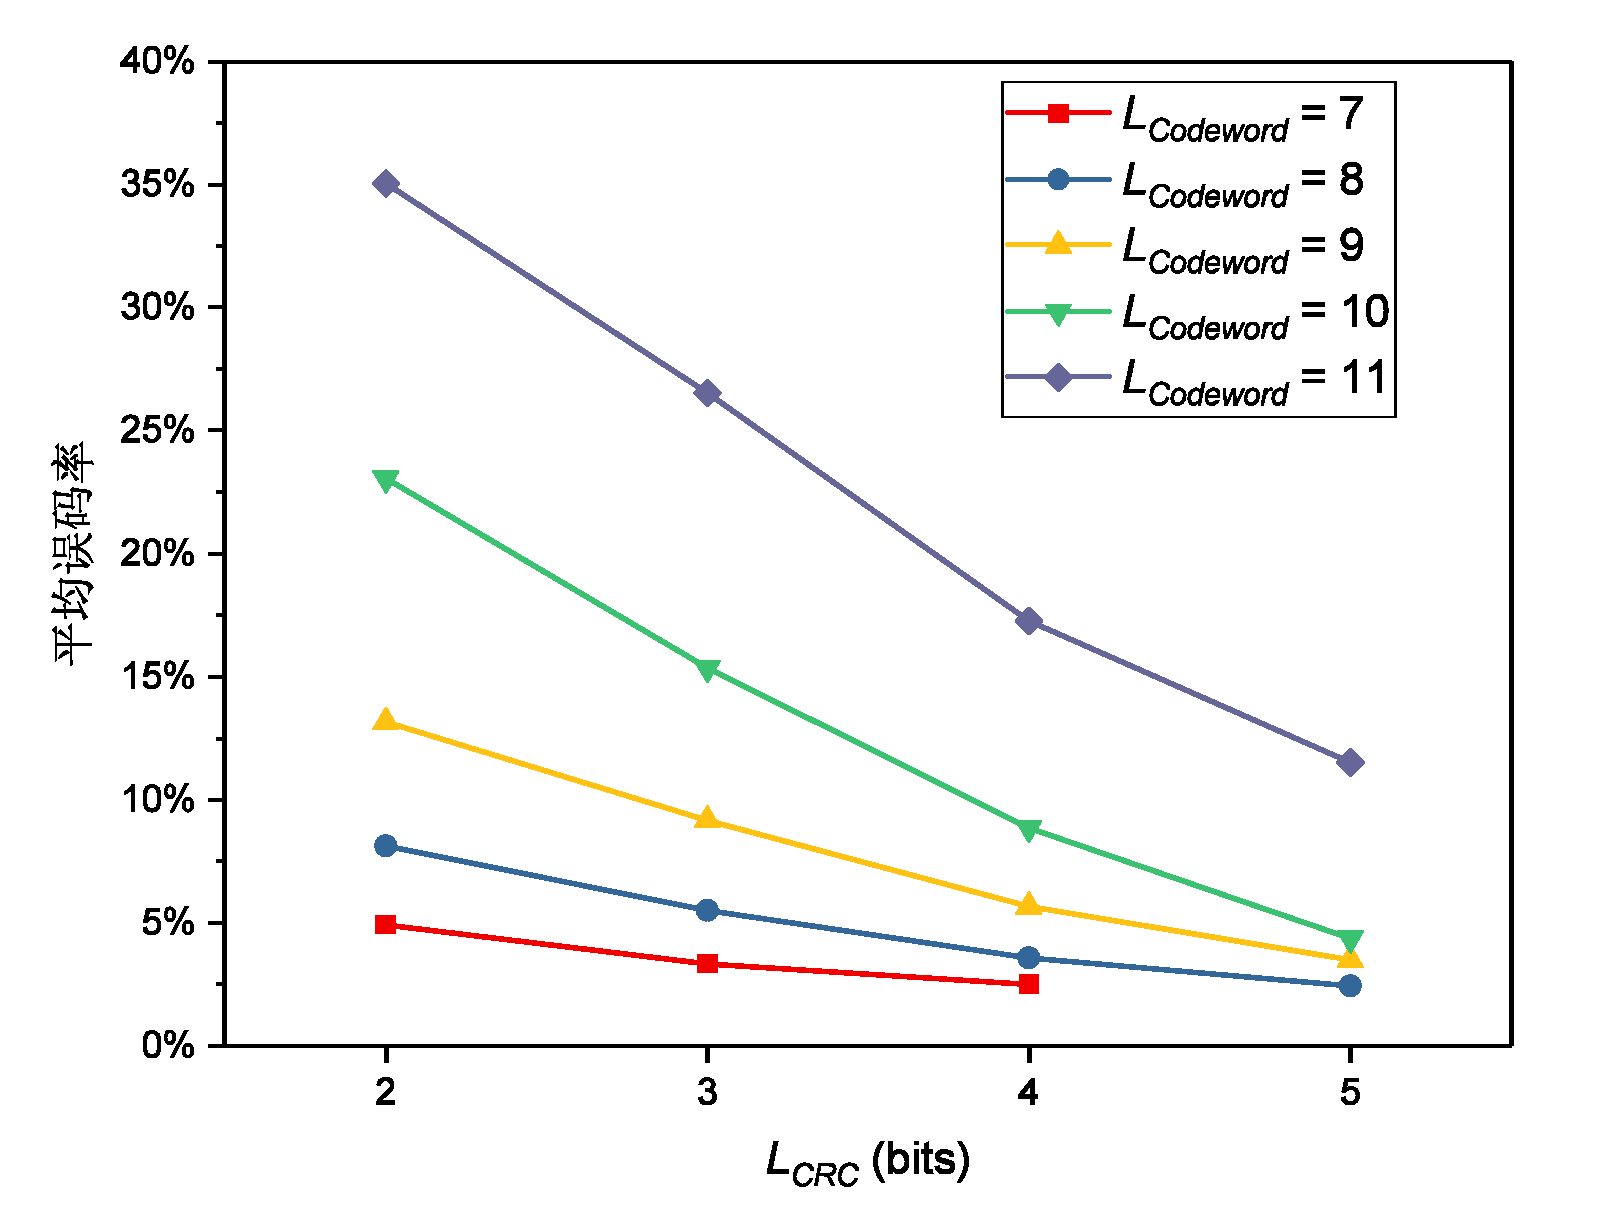
\includegraphics[width=0.48\textwidth]{chapters/chapter5/figures/ber-lcrc-good.pdf}
        }
        \caption{平均误码率与$L_{CRC}$的折线图}
        \label{fig:5:result:ber:lcrc}
    \end{figure}

    \begin{figure}[htb]
        \centering
        \subfigure[Excellent场景的平均误码率]{
            \label{fig:5:result:ber:r:excellent}
            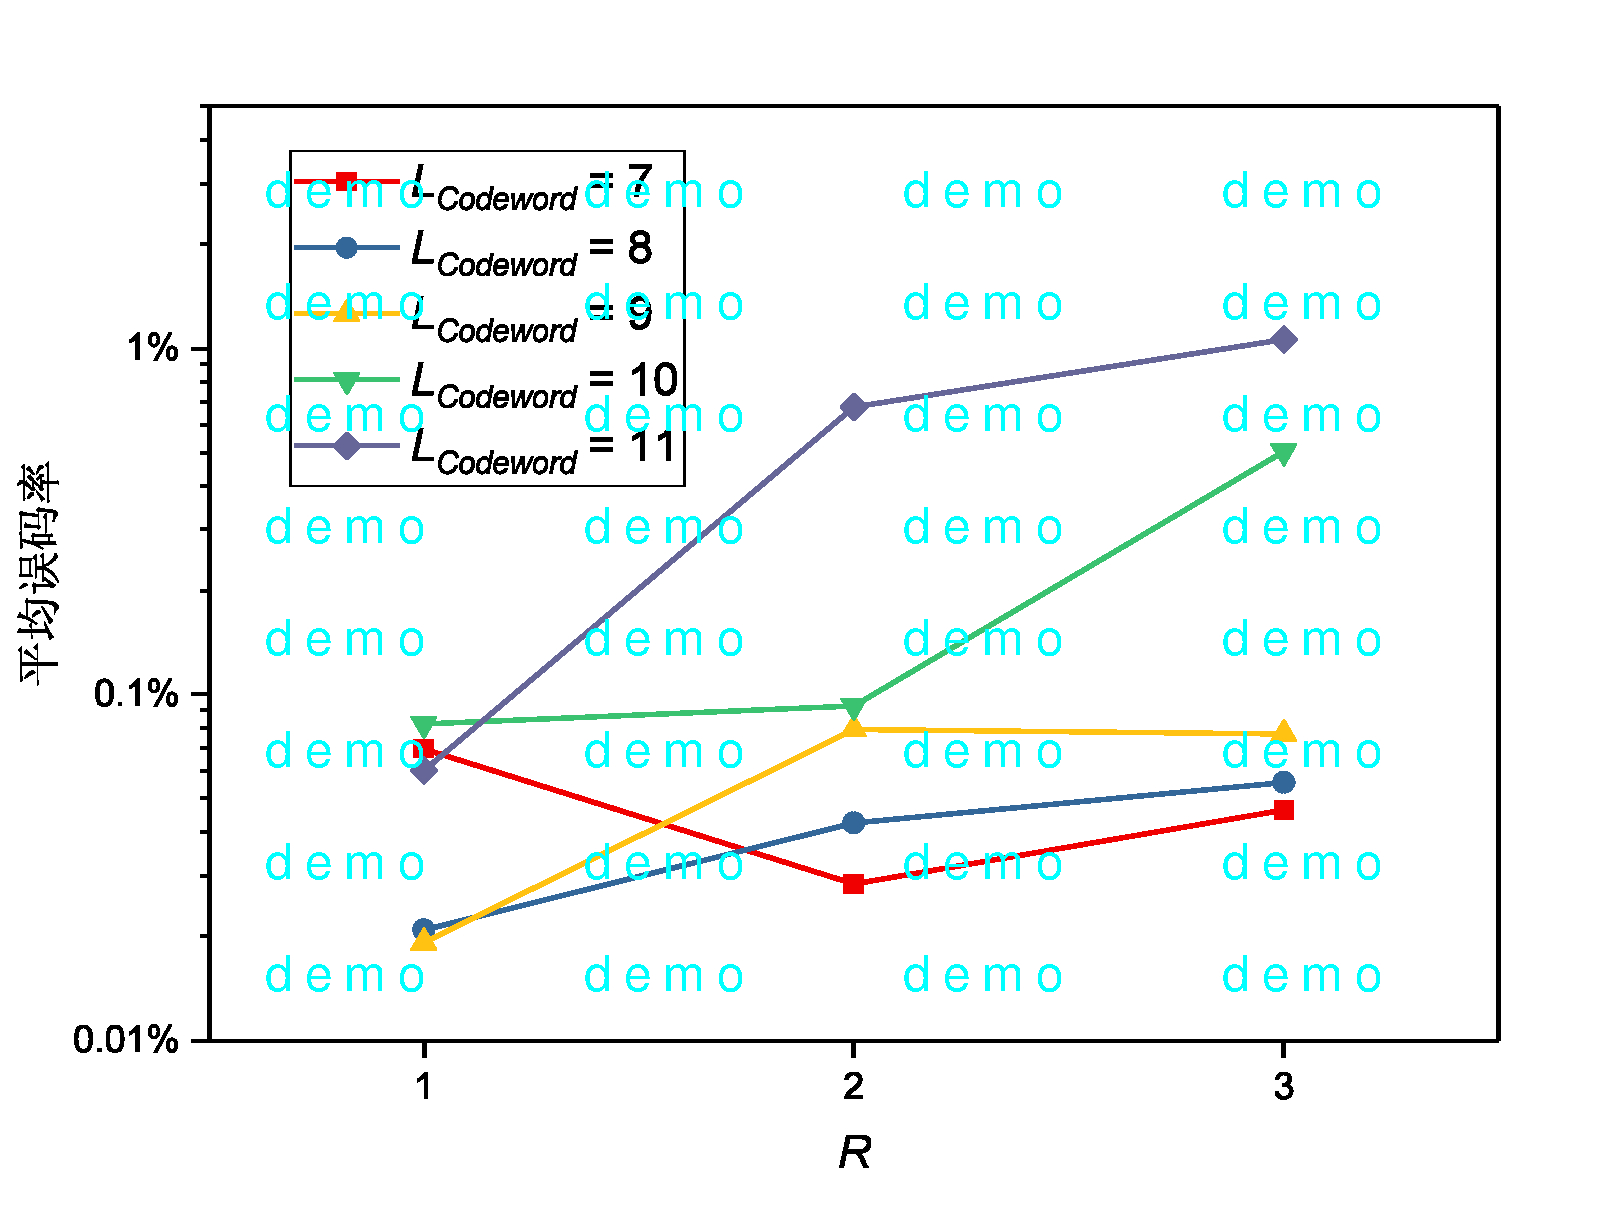
\includegraphics[width=0.48\textwidth]{chapters/chapter5/figures/ber-r-excellent.pdf}
        }
        \subfigure[Good场景的平均误码率]{
            \label{fig:5:result:ber:r:good}
            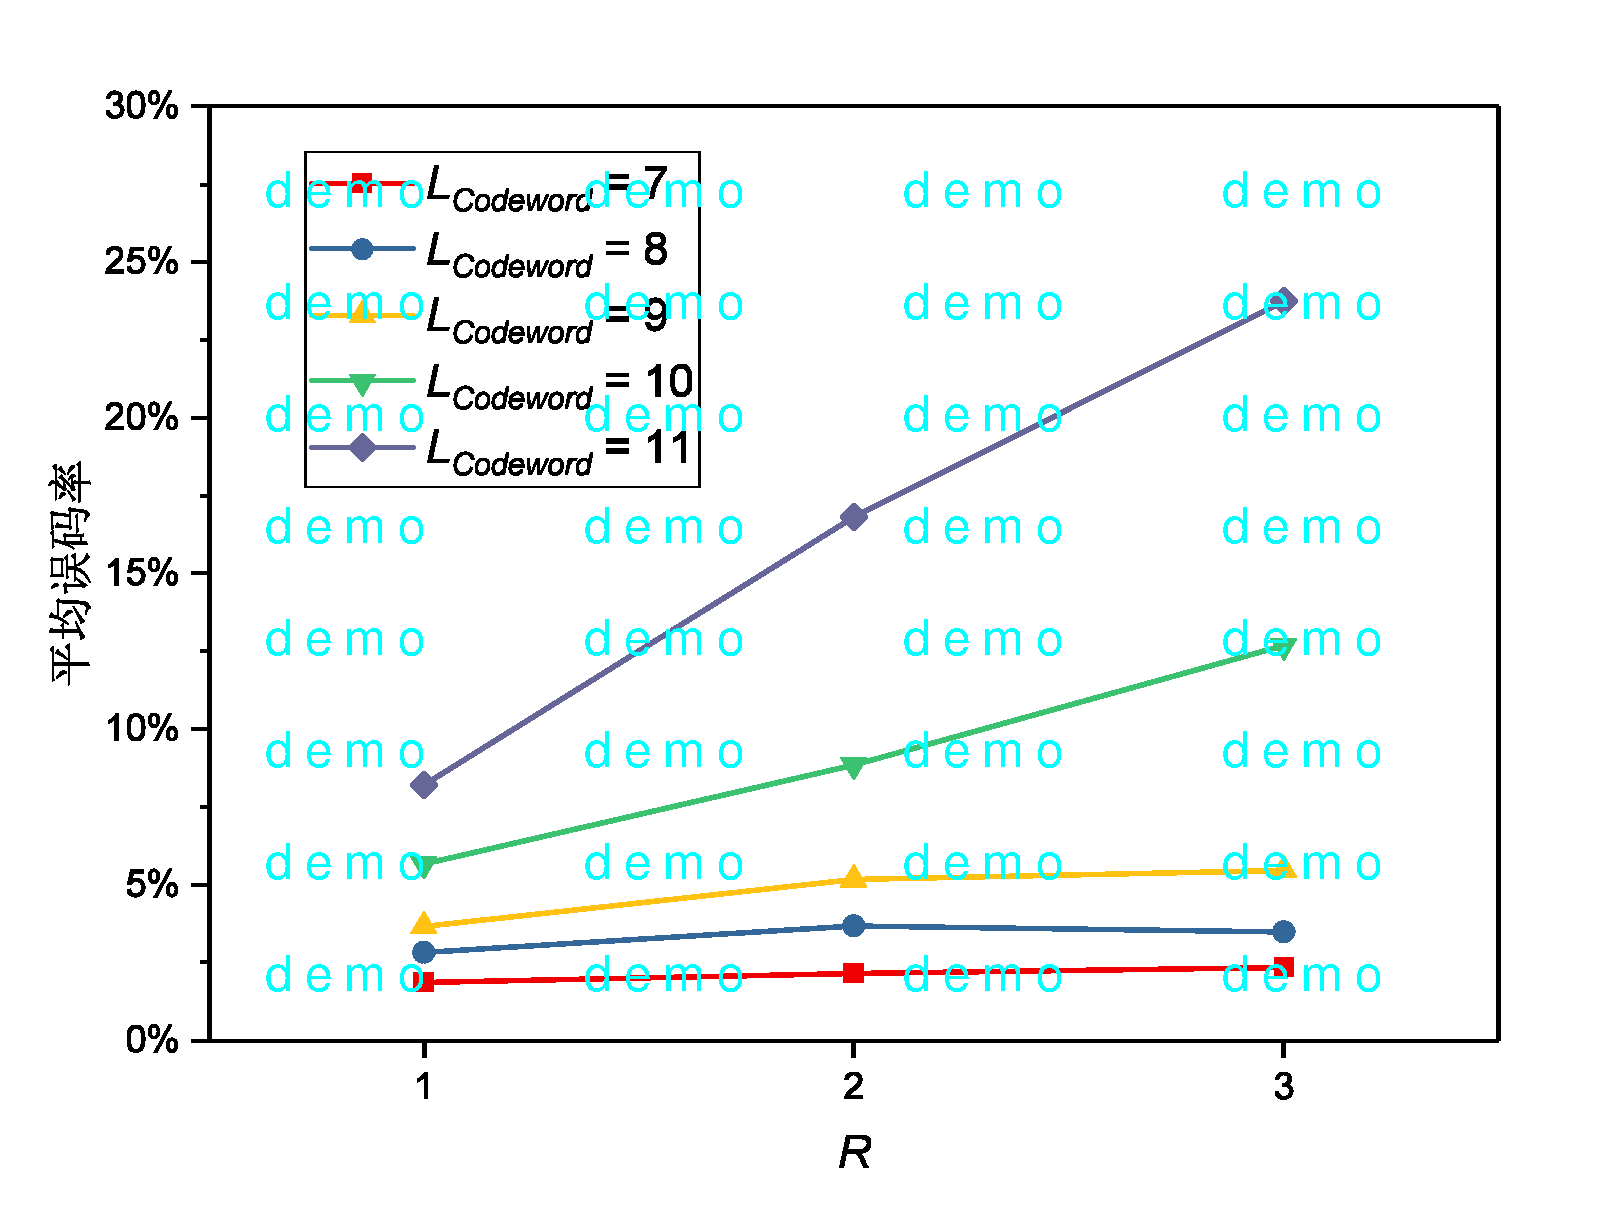
\includegraphics[width=0.48\textwidth]{chapters/chapter5/figures/ber-r-good.pdf}
        }
        \caption{平均误码率与$R$的折线图}
        \label{fig:5:result:ber:r}
    \end{figure}
}

Excellent场景及Good场景下的平均误码率,如图\ \nref{fig:5:result:ber:mcols}、图\ \nref{fig:5:result:ber:lcodeword}、图\ \nref{fig:5:result:ber:lhash}、图\ \nref{fig:5:result:ber:lcrc}及图\ \nref{fig:5:result:ber:r}。其中,图\ \nref{fig:5:result:ber:mcols}为平均误码率与参数$M_{cols}$的关系。图\ \nref{fig:5:result:ber:mcols:excellent}中,Excellent场景下误码率水平已经较低,增大$M_{cols}$能够在一定程度上降低平均误码率。图\ \nref{fig:5:result:ber:mcols:good}中,Good场景下误码率水平较高,增大$M_{cols}$产生的效果有限。

图\ \nref{fig:5:result:ber:lcodeword}中,维持$L_{HASH}\ +\ L_{CRC}$不变的情况下,增大$L_{Codeword}$导致误码率增加。由于{$L_{Codeword}$\ bits}数据对应的数据包数量为$2^{L_{Codeword}}$,$L_{Codeword}$每增加{1\ bit},数据包数量翻倍,相同丢包率下每组的噪声强度也相应加倍。因此,要达到较好的鲁棒性,参数$L_{Codeword}$要尽可能减小。

图\ \nref{fig:5:result:ber:lhash}中,平均误码率随着$L_{HASH}$增大而减小,并且Good场景中平均误码率改善效果较好。类似的,图\ \nref{fig:5:result:ber:lcrc}中,平均误码率随着$L_{CRC}$增大而减小。Excellent场景中,平均误码率已经处于较低水平,增大$L_{HASH}$及$L_{CRC}$产生的效果有限;而Good场景中,随着$L_{HASH}\ +\ L_{CRC}$的增加,平均误码率快速下降。另一方面,一定程度上增大$L_{Codeword}$,码字中能够容纳更多的校验位数,因此在改善鲁棒性方面存在一定的积极意义。

图\ \nref{fig:5:result:ber:r}中,随着参数$R$的增大,平均误码率增长。由于$R$决定了基于HASH的码字间校验的复位周期,$R$越大则复位周期越长,噪声的累积效应对鲁棒性影响越大。

\insertFigure{
	\begin{figure}[htbp]
        \centering
        \subfigure[$L_{Codeword}$与平均误码率]{
            \label{fig:5:result:ber:random:lcodeword}
            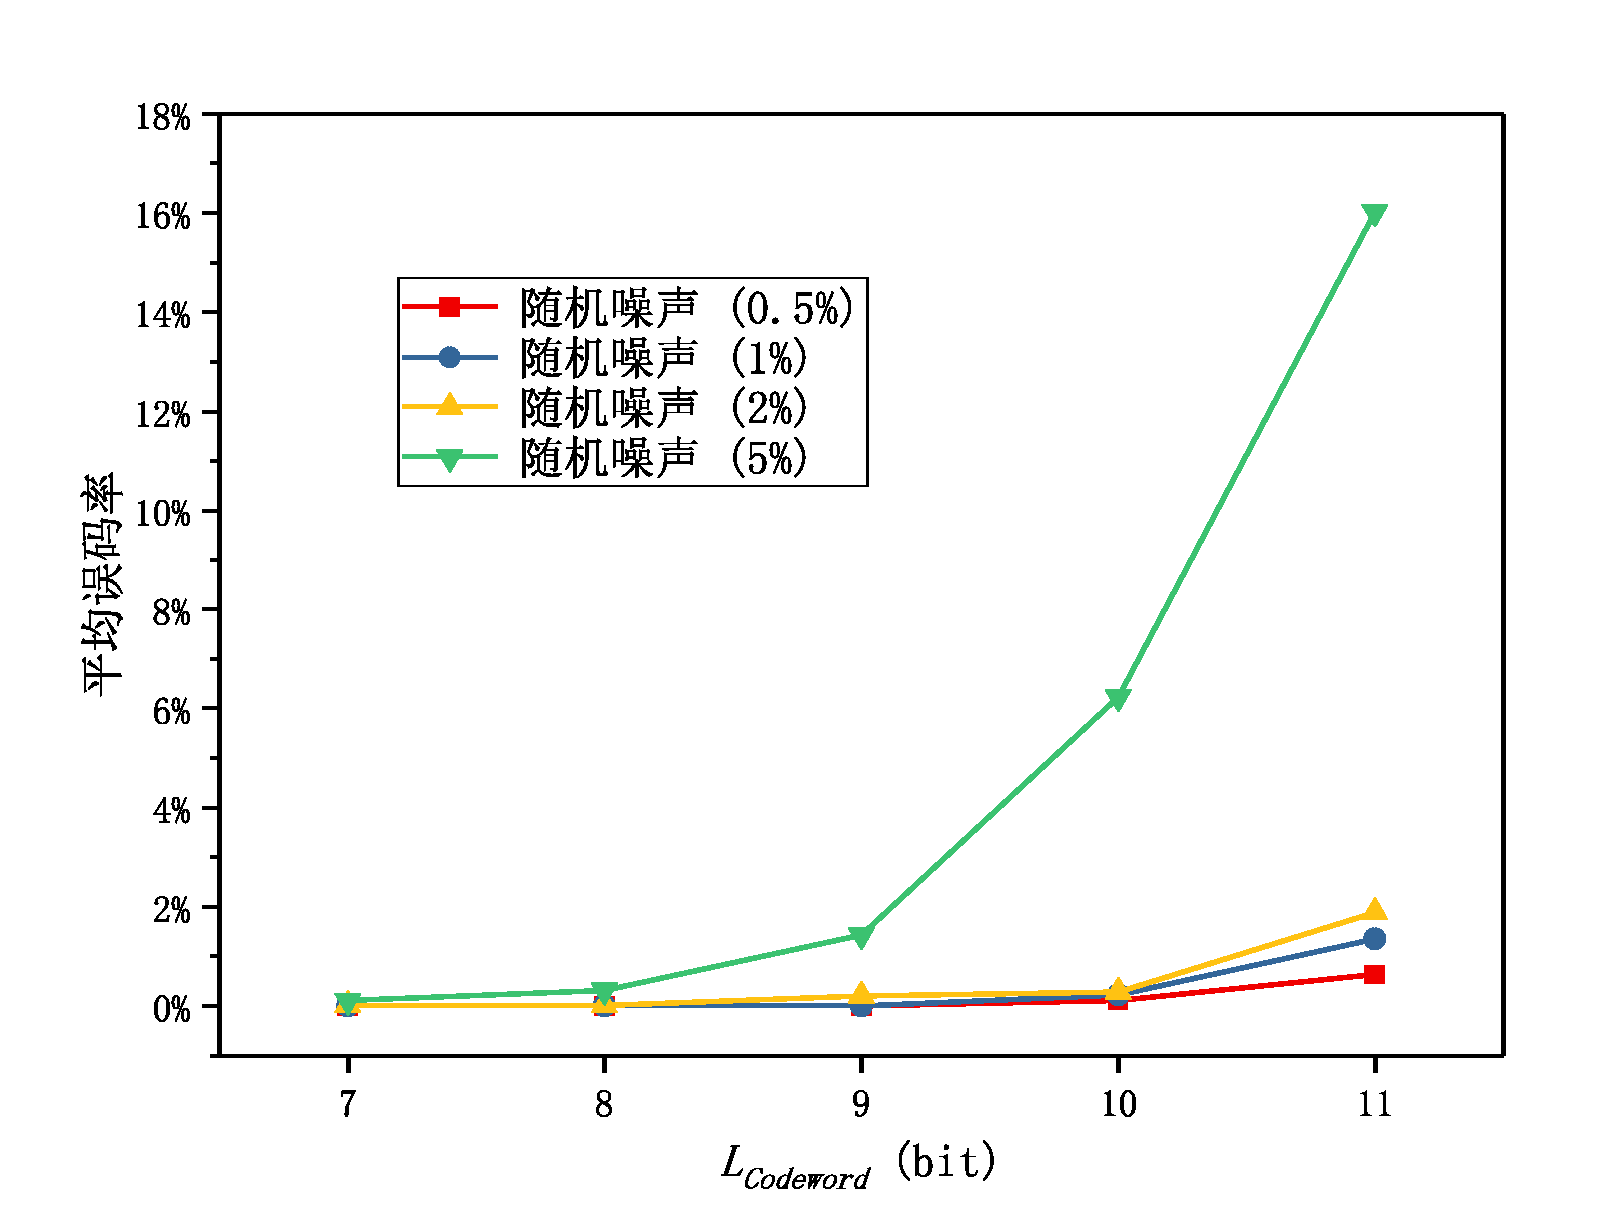
\includegraphics[width=0.48\textwidth]{chapters/chapter5/figures/ber-lcodeword-random.pdf}
        }
        \subfigure[$L_{HASH}$与平均误码率]{
            \label{fig:5:result:ber:random:lhash}
            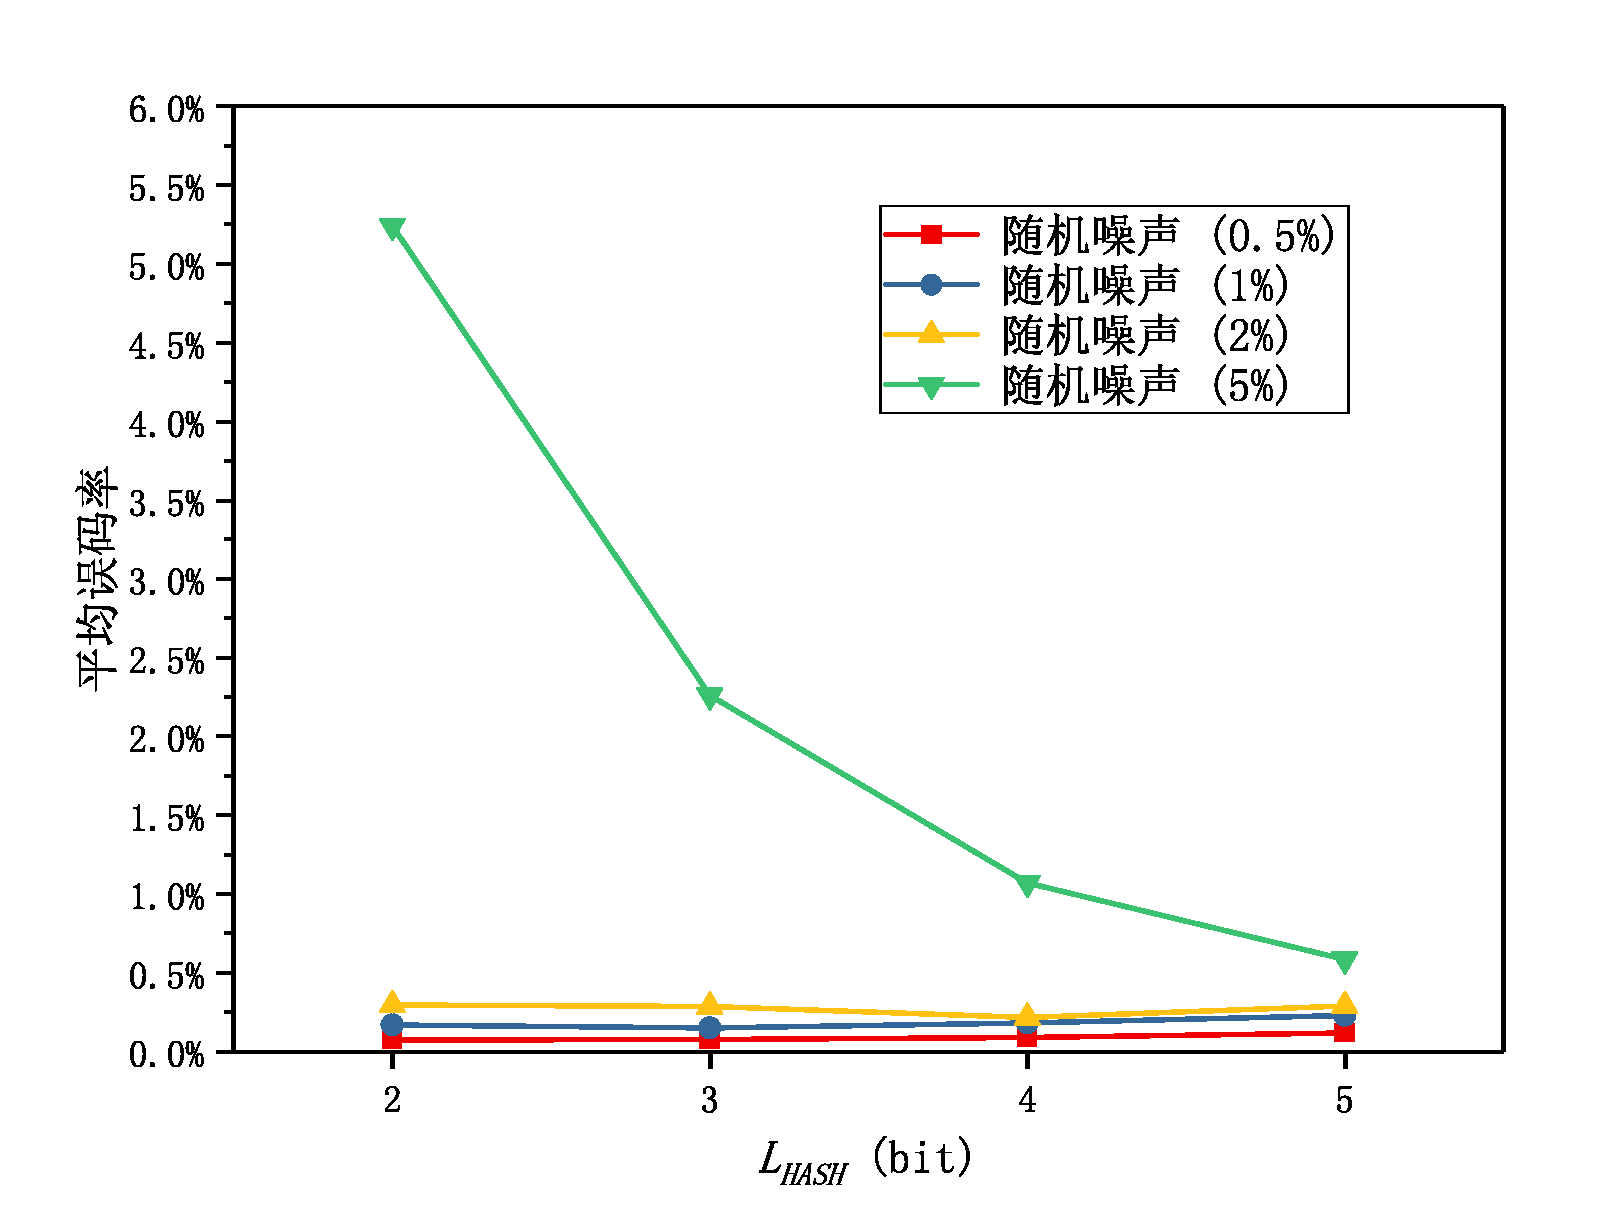
\includegraphics[width=0.48\textwidth]{chapters/chapter5/figures/ber-lhash-random.pdf}
        }
        \subfigure[$L_{CRC}$与平均误码率]{
            \label{fig:5:result:ber:random:lcrc}
            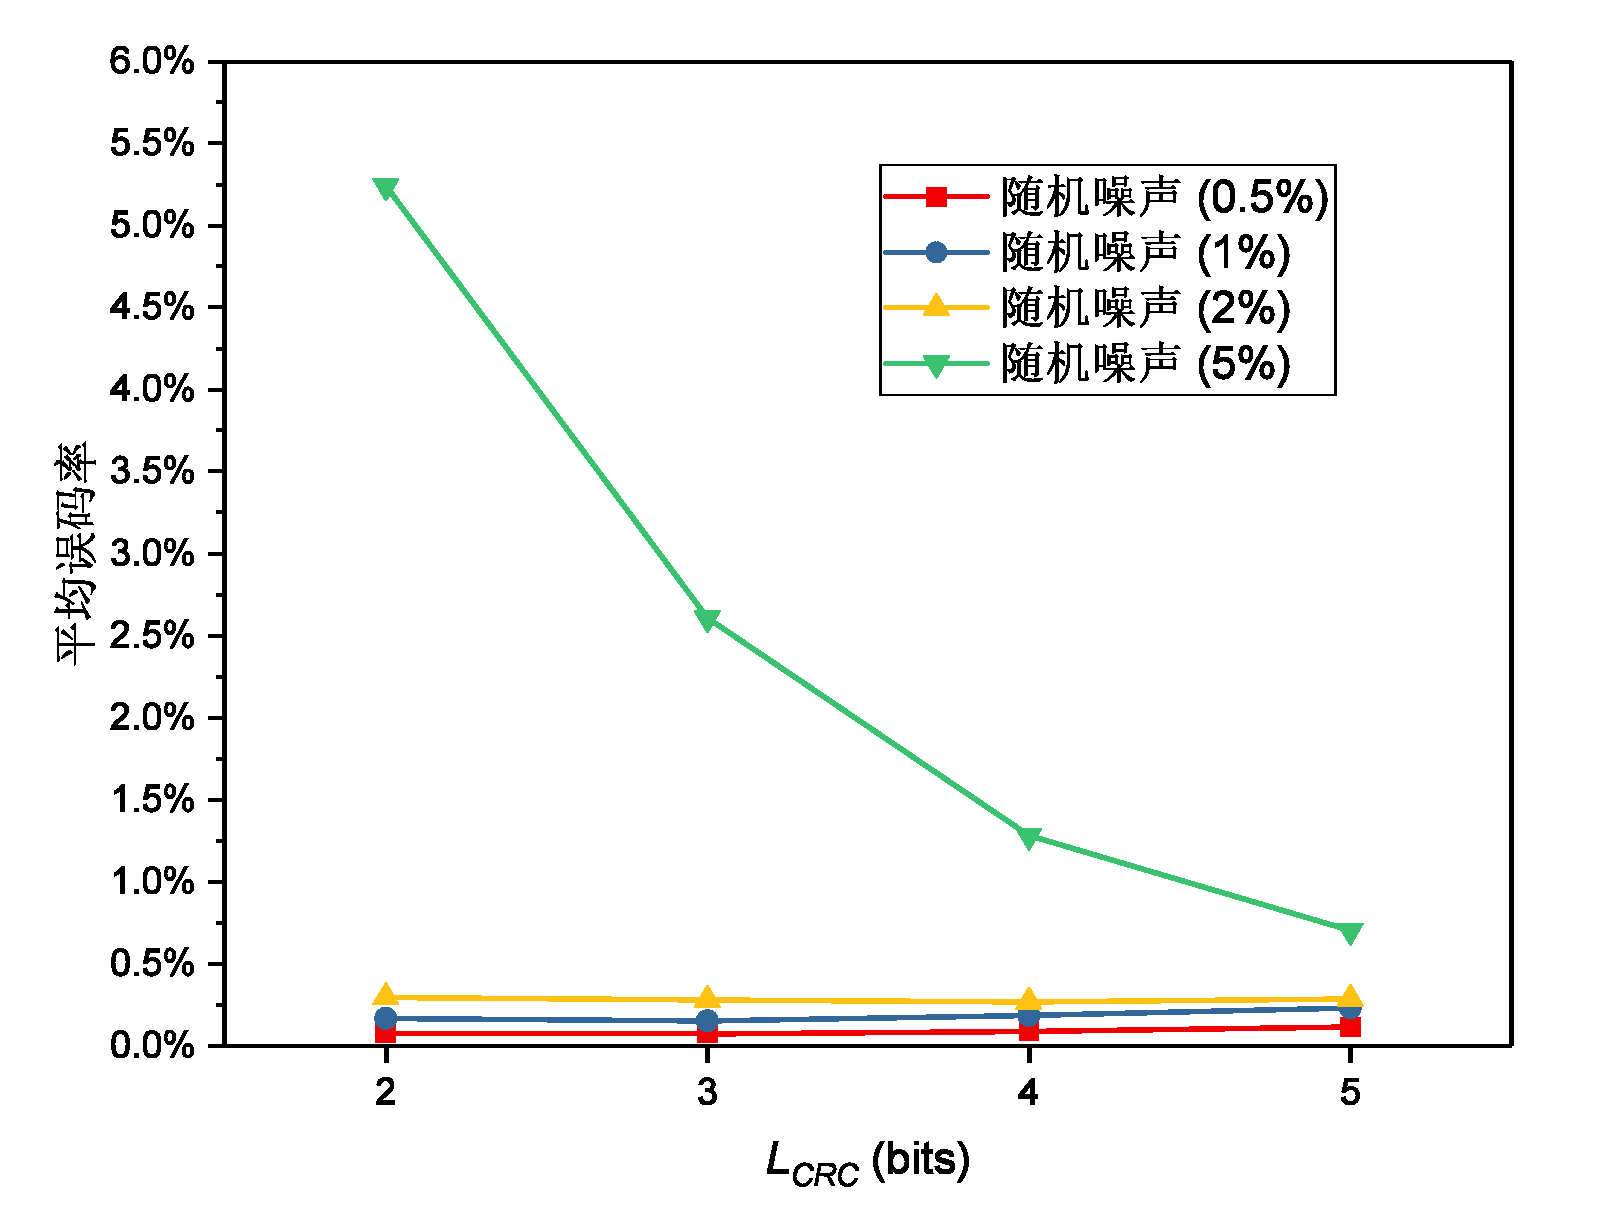
\includegraphics[width=0.48\textwidth]{chapters/chapter5/figures/ber-lcrc-random.pdf}
        }
        \subfigure[$R$与平均误码率]{
            \label{fig:5:result:ber:random:r}
            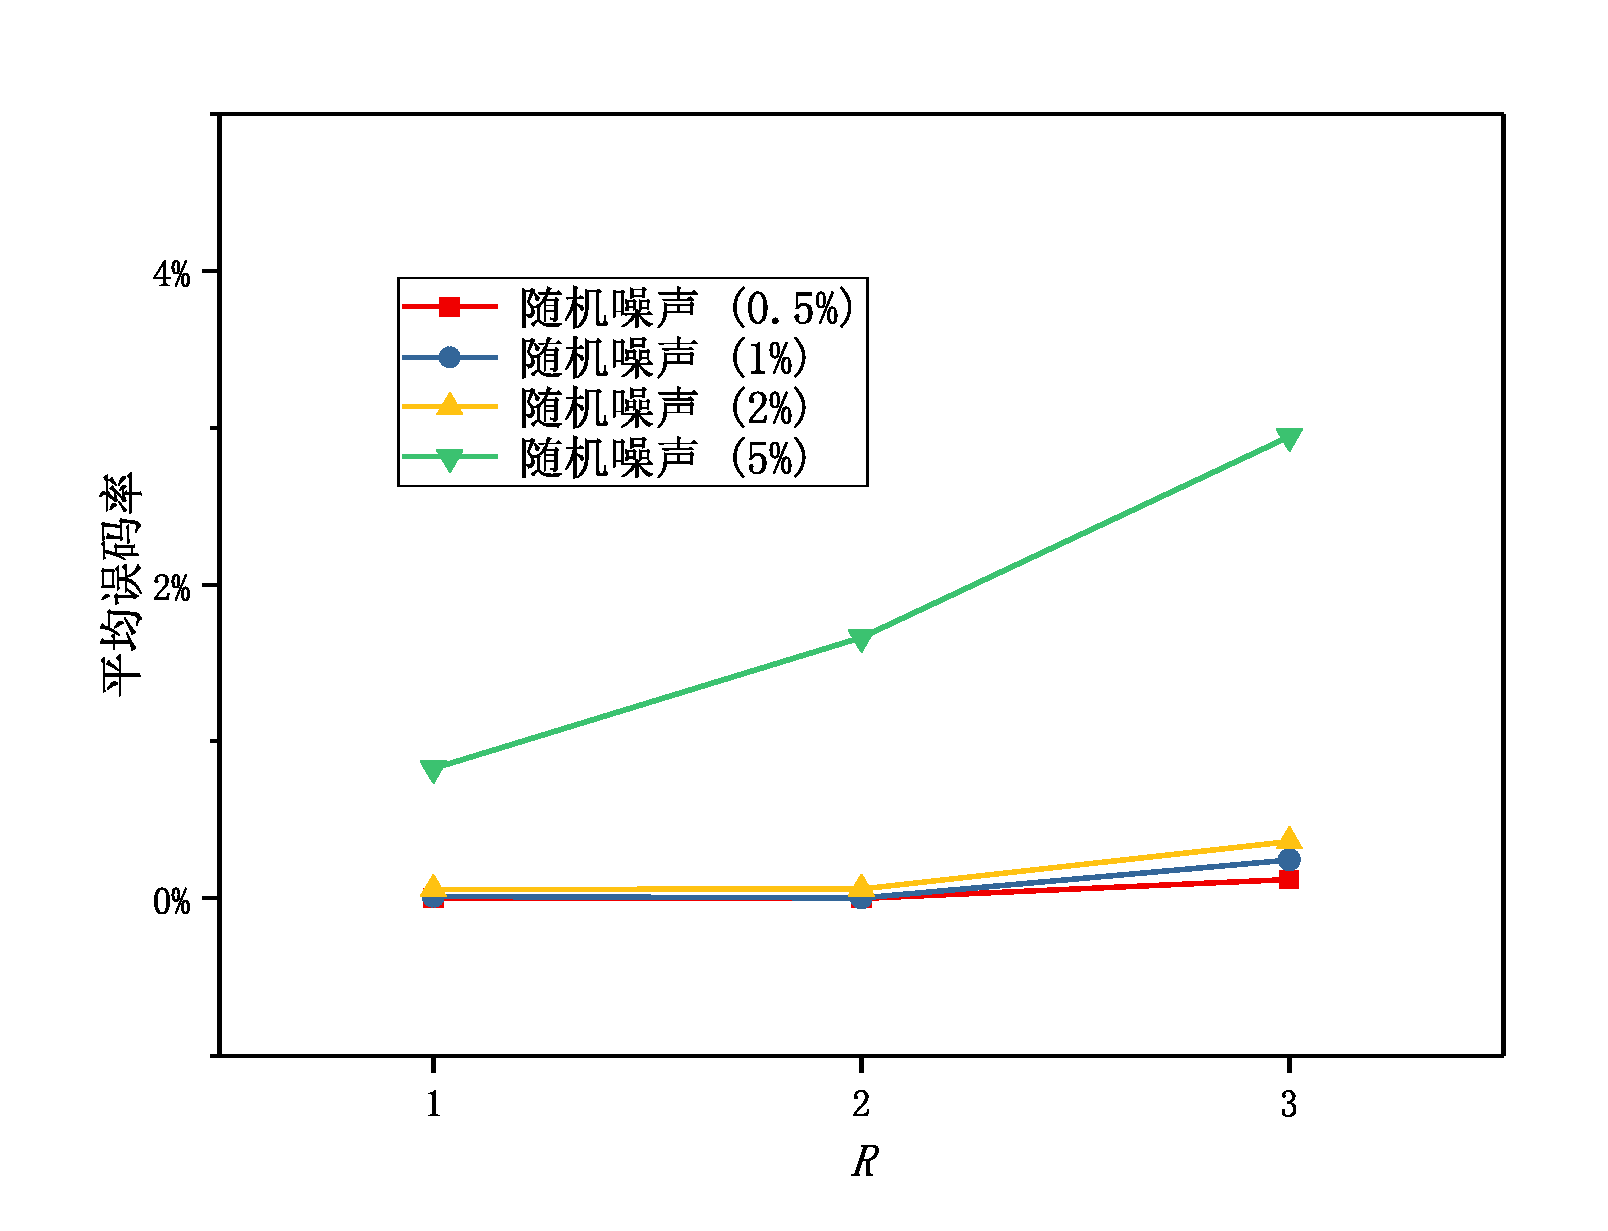
\includegraphics[width=0.48\textwidth]{chapters/chapter5/figures/ber-r-random.pdf}
        }
        \caption{随机噪声场景中平均误码率与参数关系的折线图}
        \label{fig:5:result:ber:random}
    \end{figure}
}

随机噪声场景中,鲁棒性测试结果如图\ \nref{fig:5:result:ber:random}。图\ \nref{fig:5:result:ber:random}中,当随机丢包率小于{$2\ \%$}时,平均误码率变化较小,证明鲁棒性方法已经足够应对噪声影响。直至随机丢包噪声为{$5\ \%$}时,平均误码率曲线才随参数变化出现波动。

通过两种模式下的测试,对于该时间隐通道的参数,增大$M_{cols}$、减小$L_{Codeword}$、增大$L_{HASH}$、增大$L_{CRC}$及减小$R$均可降低误码率。根据公式(\nref{equ:5:codeword-length}),每个码字中含有的数据位数$BL$,与码字长度$L_{Codeword}$、HASH校验位数$L_{HASH}$及CRC校验位数$L_{CRC}$存在密切关系,提高鲁棒性对抗检测能力及传输性能均产生影响,参数配置需要综合考虑。

\subsection{传输性能测试}
\label{chap:hash:result:throughput}

根据该时间隐通道的设计方案,参数$L_{Codeword}$、$L_{HASH}$、$L_{CRC}$及$R$均影响传输性能。时间隐通道容量与参数的关系如公式(\nref{equ:5:capacity}),时间隐通道传输速率与参数的关系如公式(\nref{equ:5:throughput})。
\insertEquation{
    \begin{equation}
    \label{equ:5:capacity}
    \begin{split}
        Capacity\ &=\ \frac{BL\ \times\ R}{(R+1)\ \times\ 2^{L_{Codeword}}}\ \times\ \frac{2}{3}\quad (bpp)\ \\
        &=\ \frac{(L_{Codeword}\ -\ L_{HASH}\ -\ L_{CRC})\ \times\ R}{(R\ +\ 1)\ \times\ 2^{L_{Codeword}}}\ \times\ \frac{2}{3}\quad (bpp)
    \end{split}
    \end{equation}
    \begin{equation}
    \label{equ:5:throughput}
    \begin{split}
        Throughput\ &=\ Capacity\ \times\ 100\ \times\ \frac{2}{3}\quad (bps)\ \\
        &=\ \frac{(L_{Codeword}\ -\ L_{HASH}\ -\ L_{CRC})\ \times\ R\ \times\ 100}{(R\ +\ 1)\ \times\ 2^{L_{Codeword}}}\ \times\ \frac{2}{3}\quad (bps)
    \end{split}
    \end{equation}
}
\insertFigure{
	\begin{figure}[htbp]
        \centering
        \subfigure[$L_{HASH}+L_{CRC}=4$时的传输速率]{
            \label{fig:5:result:bps-4}
            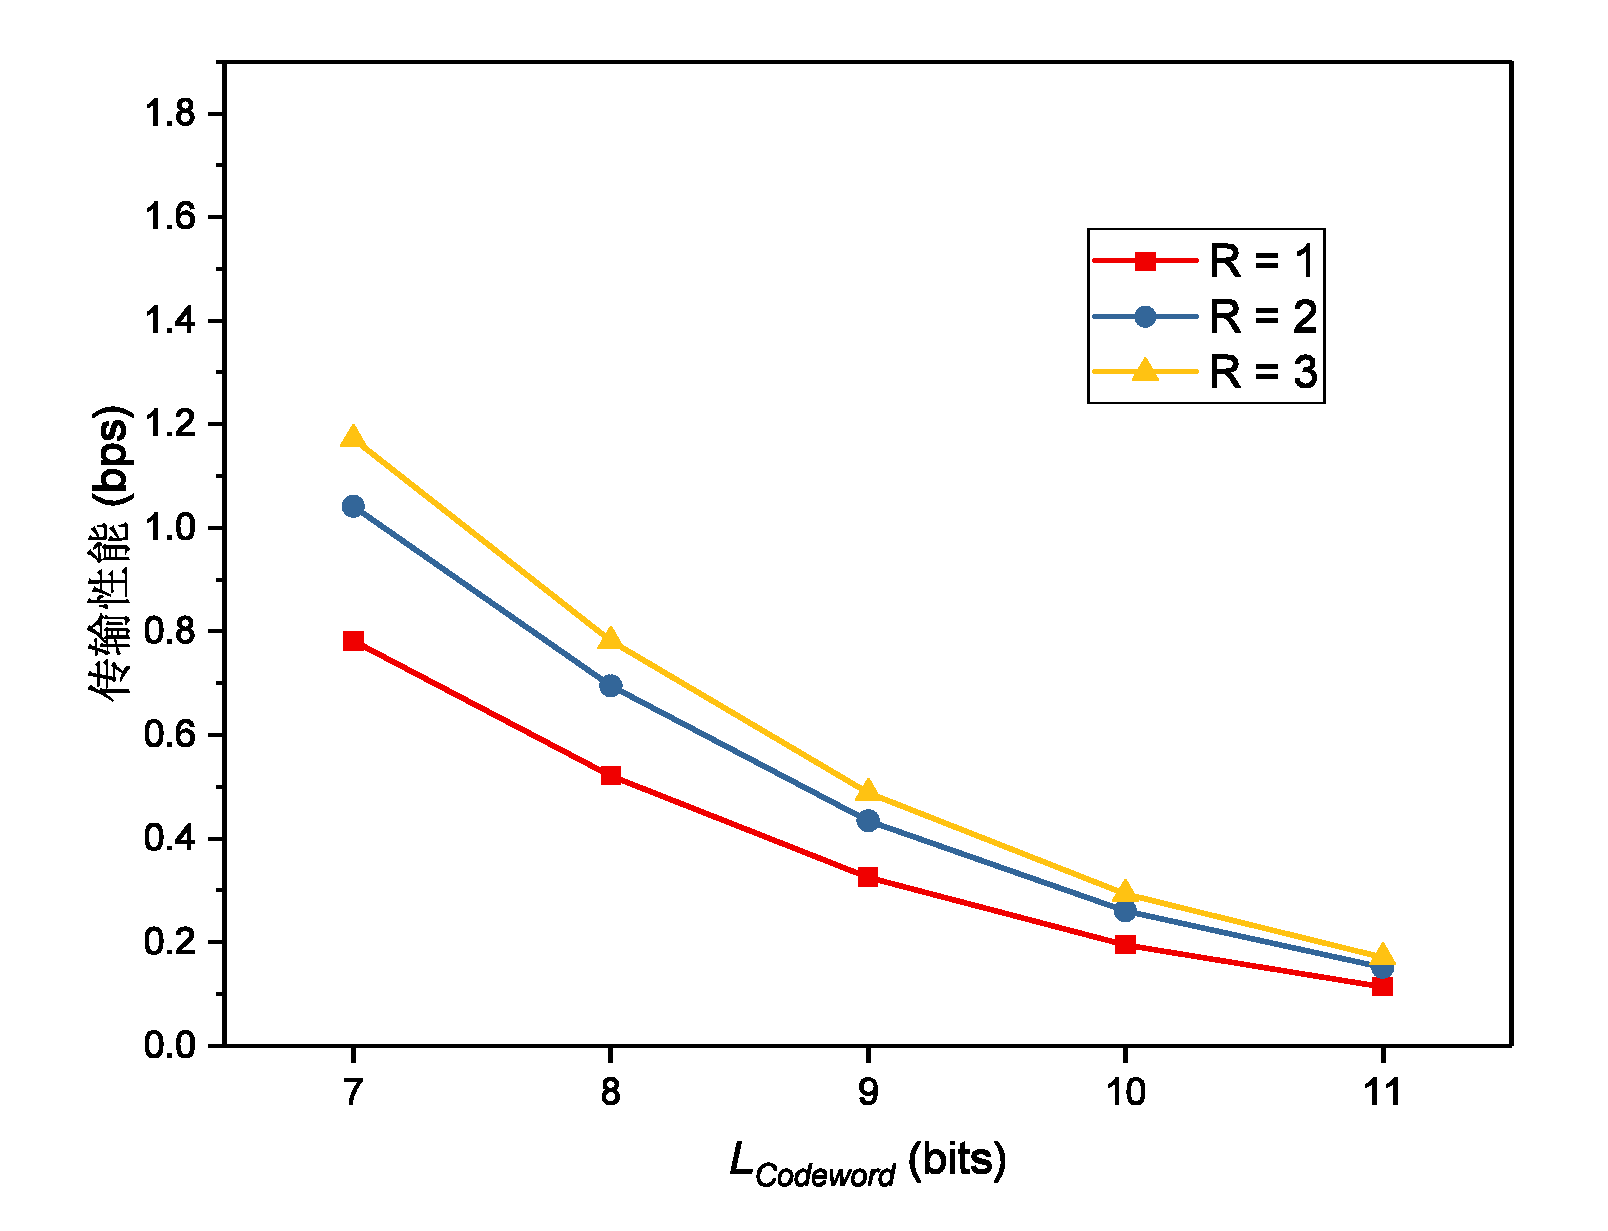
\includegraphics[width=0.48\textwidth]{chapters/chapter5/figures/bps-4.pdf}
        }
        \subfigure[$L_{HASH}+L_{CRC}=6$时的传输速率]{
            \label{fig:5:result:bps-6}
            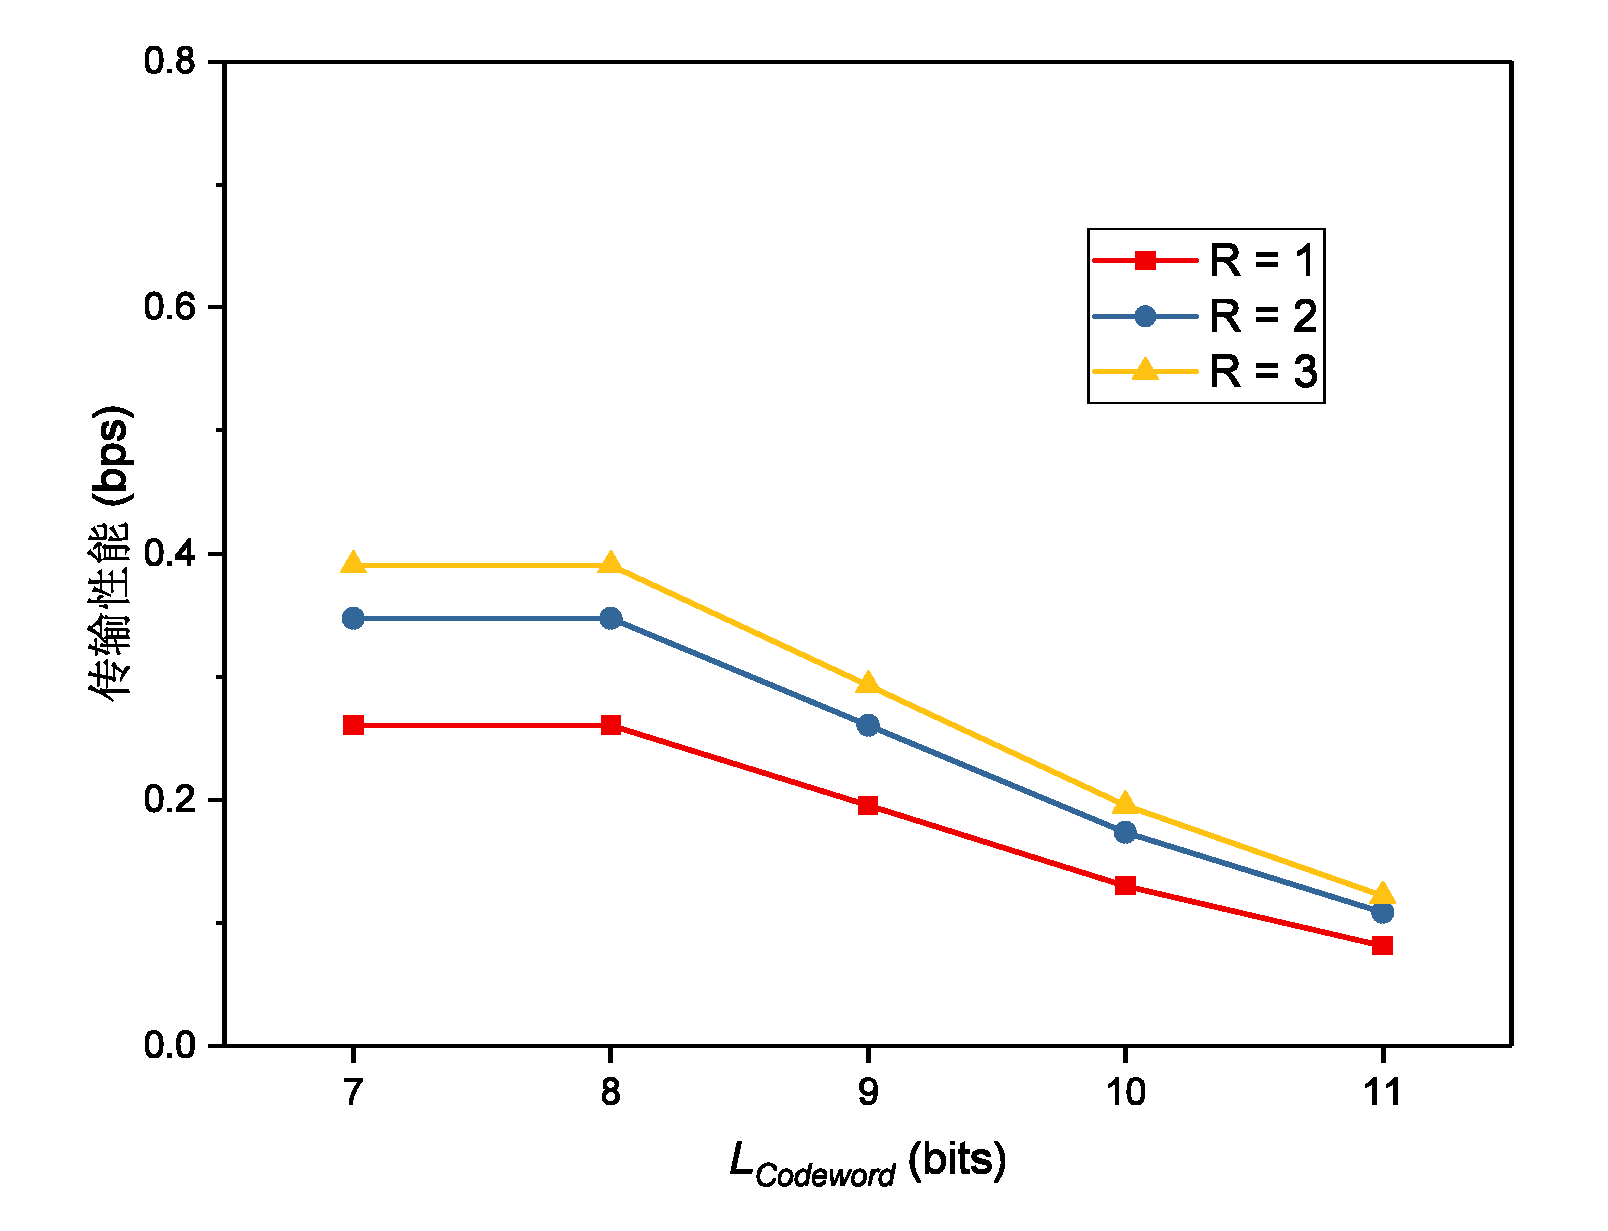
\includegraphics[width=0.48\textwidth]{chapters/chapter5/figures/bps-6.pdf}
        }
        \caption{时间隐通道传输速率与$L_{Codeword}$及$R$的关系图}
        \label{fig:5:result:bps}
    \end{figure}
}

当$L_{HASH}\ +\ L_{CRC}\ =\ 4$时,时间隐通道的传输速率与$L_{Codeword}$及$R$的关系如图\ \nref{fig:5:result:bps-4}。当$L_{HASH}\ +\ L_{CRC}\ =\ 6$时,时间隐通道的传输速率与$L_{Codeword}$及$R$的关系如图\ \nref{fig:5:result:bps-6}。Excellent场景中,传输性能可达到{1.0\ bps}。通过增大复位周期$R$,能够在一定水平上提升传输速率,但远小于降低$L_{HASH}\ +\ L_{CRC}$带来的性能提升。

\subsection{构建代价测试}
\label{chap:hash:result:cost}

\insertFigure{
	\begin{figure}[htbp]
        \centering
        \subfigure[Excellent场景的视频质量]{
            \label{fig:5:result:vq-excellent}
            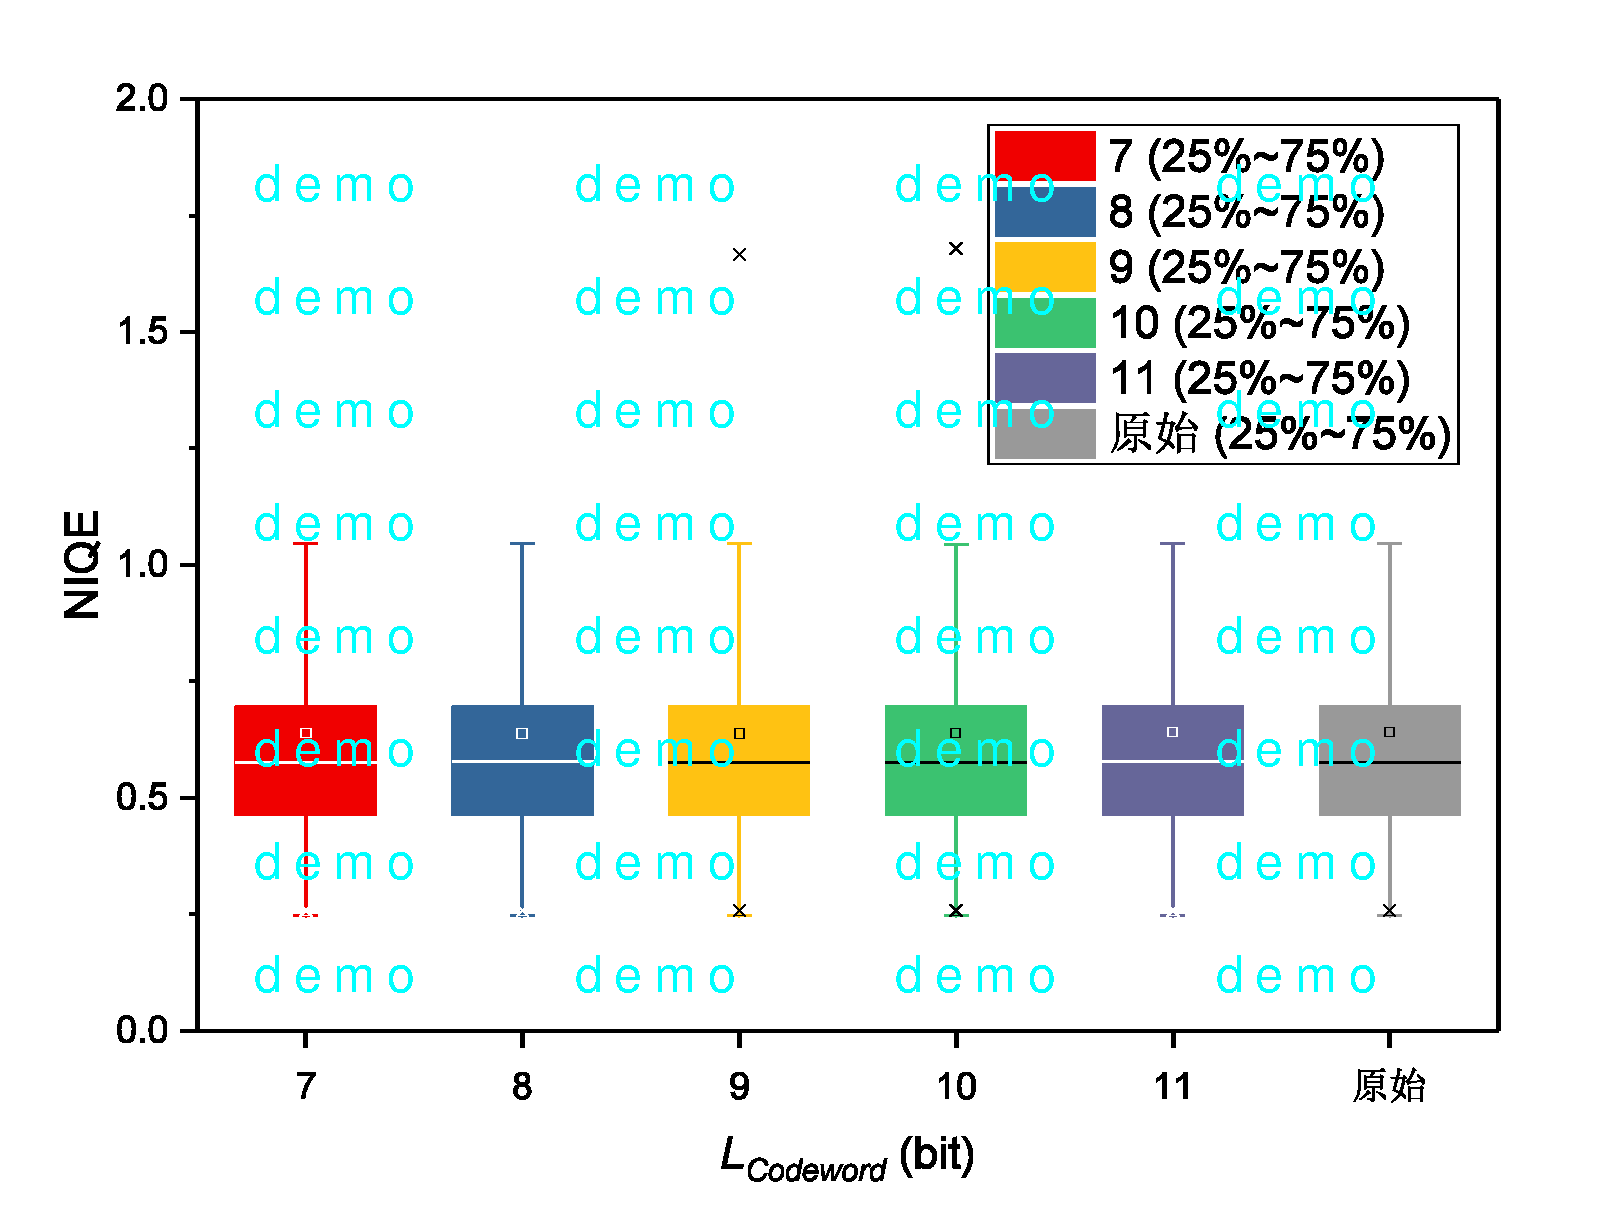
\includegraphics[width=0.48\textwidth]{chapters/chapter5/figures/vq-excellent.pdf}
        }
        \subfigure[Good场景的视频质量]{
            \label{fig:5:result:vq-good}
            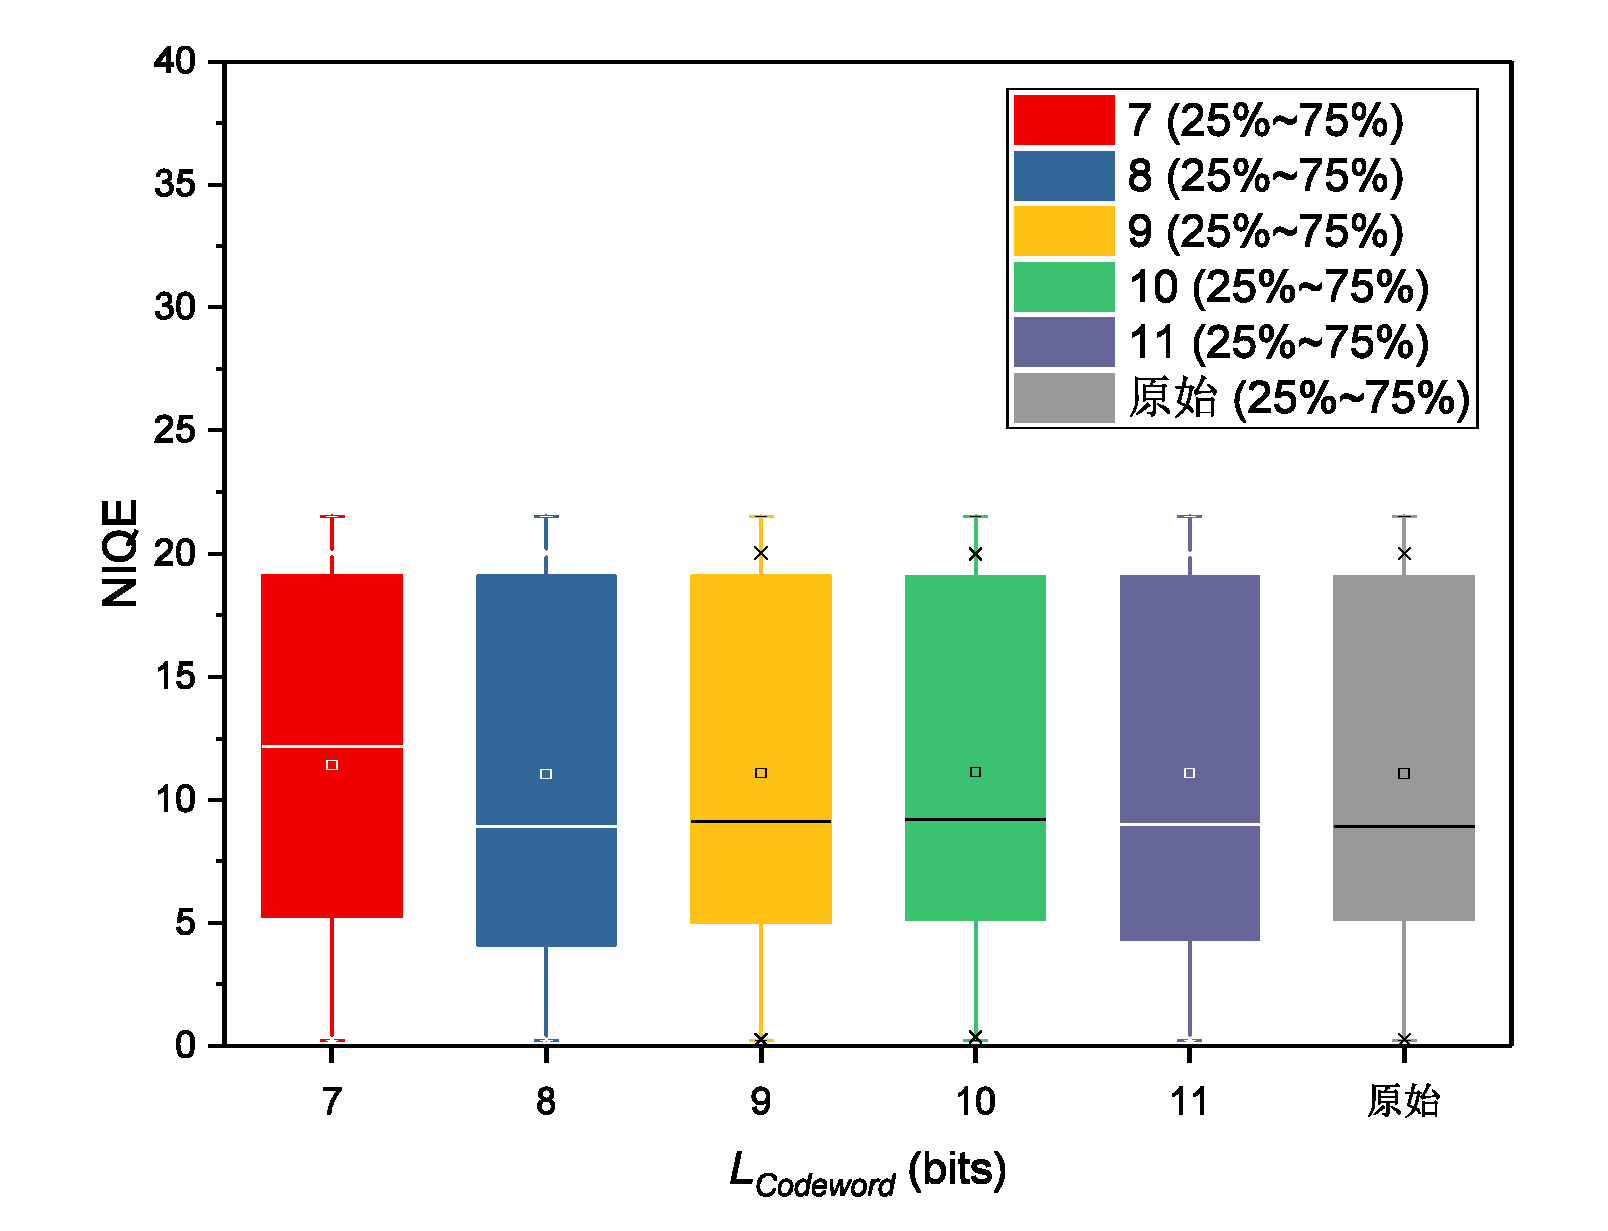
\includegraphics[width=0.48\textwidth]{chapters/chapter5/figures/vq-good.pdf}
        }
        \caption{时间隐通道的NIQE视频质量评估结果}
        \label{fig:5:result:vq}
    \end{figure}
}

该时间隐通道的构建代价测试,主要评估时间隐通道对视频质量的影响,评估指标采用NIQE(Natural Image Quality Evaluator)无参照指标\nupcite{7094273},NIQE值与视频质量呈负相关。时间隐通道的NIQE评估结果如图\ \nref{fig:5:result:vq},两种场景中由于网络噪声强度的差异,视频质量已经存在较大差距。图\ \nref{fig:5:result:vq-excellent},Excellent场景下,不同$L_{Codeword}$下的NIQE值相似,且波动较小。图\ \nref{fig:5:result:vq-good},Good场景下,时间隐通道导致NIQE值产生波动,但无较大的分布差异。通过对比图\ \nref{fig:5:result:vq-excellent}及图\ \nref{fig:5:result:vq-good},相较时间隐通道导致的视频质量损失,网络噪声导致的视频质量损失影响更大,因此该时间隐通道的构建代价可接受。

\subsection{测试结果总结}
\label{chap:hash:result:evaluation}

通过测试该时间隐通道的抗检测能力、鲁棒性、传输性能及构建代价,各参数对指标均有影响。实际应用中,时间隐通道应当在保证传输隐蔽性的基础上,具有较好的鲁棒性和传输性能,因此需要合理配置参数。根据本文\ \nref{chap:hash:result:undetectability}的测试结果,当$L_{Codeword}\ge 9$时,即可满足抗检测能力要求。另一方面,时间隐通道作为寄生信道,受噪声干扰不可避免。因此在综合评估中,设定Excellent场景中可接受误码率在{$0.1\ \%$}以内,Good场景中可接受误码率在{$1\ \%$}以内,进而筛选参数组合。

\insertTable{
	\begin{table}[htbp]
      \centering
      \caption{基于多重校验纠错的时间隐通道参数组合评估表}
      \label{tab:5:result:results-sum}
          \begin{tabular*}{0.9\textwidth}{@{\extracolsep{\fill}}cccccccc}
            \toprule
            场景 & $M_{cols}$ & $L_{Codeword}$ & $L_{HASH}$ & $L_{CRC}$ & $R$ & 传输速率 & 平均误码率 \\
            \midrule
            \multirow{3}{*}{Excellent} 
            & 36 & 9 & 3 & 2 & 2 & 0.35\ bps & $<0.001\ \%$ \\
            & 27 & 9 & 2 & 3 & 3 & 0.40\ bps & $<0.02\ \%$ \\
            & 27 & 9 & 2 & 2 & 3 & 0.49\ bps & $<0.08\ \%$ \\
            \\
            \multirow{3}{*}{Good} 
            & 45 & 9 & 5 & 2 & 1 & 0.13\ bps & $<0.85\ \%$ \\
            & 36 & 10 & 5 & 3 & 3 & 0.10\ bps & $<0.10\ \%$ \\
            & 45 & 10 & 5 & 4 & 2 & 0.05\ bps & $<0.01\ \%$ \\
            \bottomrule
          \end{tabular*}
    \end{table}
}

该时间隐通道的综合评估结果如表\ \nref{tab:5:result:results-sum},通过对比试验结果,筛选出Excellent场景及Good场景中效果较好的参数配置。由表可见,Excellent场景中牺牲一定的鲁棒性,能够取得更好的性能表现。Good场景中,需要较多的鲁棒性信息抵御噪声干扰,因此牺牲性能才可保证传输可靠性。

\insertTable{
	\begin{table}[htbp]
      \centering
      \caption{基于多重校验纠错的时间隐通道横向比较}
      \label{tab:5:result:compare}
          \begin{tabular*}{0.85\textwidth}{@{\extracolsep{\fill}}cccc}
            \toprule
            时间隐通道构建方法 & 传输性能 & 信道容量 & 误码率 \\
            \midrule
            SCC\nupcite{10.1007/978-3-642-16435-4_15} & & 0.2$\sim$ 0.8 bpp & 2\ \% \\
            AFTC\nupcite{7347395} & & 0.5 bpp & 4\ \% \\
            CoCo\nupcite{10.1007/978-3-642-24178-9_22} & & 0.1$\sim$ 0.5 bpp & 4\ \% \\
            SPCC\nupcite{8288828} & 0.7$\sim$ 3 bps & & 0.9\ \% \\
            Zigzag-CTC & 0.88 bps & 0.009 bpp & 1.5\ \% \\
            MSV-CTC & 0.49 bps & 0.005 bpp & 0.08\ \% \\
            \bottomrule
          \end{tabular*}
    \end{table}
}

表\ \nref{tab:5:result:compare}对比了几种时间隐通道的性能及误码率水平,分别为SCC\nupcite{10.1007/978-3-642-16435-4_15}、AFTC\nupcite{7347395}、CoCo\nupcite{10.1007/978-3-642-24178-9_22}、SPCC\nupcite{8288828}、本文\ \nref{chap:zigzag:model}基于Zigzag映射矩阵的时间隐通道Zigzag-CTC,及本时间隐通道构建方法MSV-CTC(Multi-Stage Verification Covert Timing Channel)。对比可见,虽然该方法损失了部分性能,但较其它时间隐通道在鲁棒性方面有了提升。

根据抗检测能力测试、鲁棒性测试、传输性能测试及鲁棒性测试的结果,该方法能够满足时间隐通道的指标要求。由于采用了主动丢包的调制方式,该时间隐通道在基于IPD的检测方法中具有较好的隐蔽性,并且调整参数$L_{Codeword}$后,通过了基于连续丢包数及区间丢包数的测试。通过结合多个层次的校验纠错,该时间隐通道有效提高了传输鲁棒性,误码率水平降低。通过调整传输参数组合,在传输性能达到{0.49\ bps}的情况下,误码率水平不高于{$0.08\ \%$},达到了时间隐通道的基本水准。